\documentclass[a4paper,twoside]{article}
\usepackage[T1]{fontenc}
\usepackage[bahasa]{babel}
\usepackage{graphicx}
\usepackage{graphics}
\usepackage{float}
\usepackage[cm]{fullpage}
\pagestyle{myheadings}
\usepackage{etoolbox}
\usepackage{setspace} 
\usepackage{lipsum} 
\usepackage{amssymb}% untuk symbol check
\usepackage{pifont}% untuk symbol check
\usepackage{multirow}% untul multirow pada tabel
\usepackage{listings}%untuk penulisan source code
\usepackage[obeyspaces]{url}
\usepackage{xstring}%manipulasi string, strchar, ifstreq

\graphicspath{{../DokumenSkripsi/Gambar/}}% folder tempat gambar 

\setlength{\headsep}{30pt}
\usepackage[inner=2cm,outer=2.5cm,top=2.5cm,bottom=2cm]{geometry} %margin
% \pagestyle{empty}

\makeatletter
\renewcommand{\@maketitle} {\begin{center} {\LARGE \textbf{ \textsc{\@title}} \par} \bigskip {\large \textbf{\textsc{\@author}} }\end{center} }
\renewcommand{\thispagestyle}[1]{}
\markright{\textbf{\textsc{Laporan Perkembangan Pengerjaan Skripsi\textemdash Sem. Genap 2015/2016}}}

\onehalfspacing
 
\begin{document}

\title{\@judultopik}
\author{\nama \textendash \@npm} 

%ISILAH DATA BERIKUT INI:
\newcommand{\nama}{Amabel Levint}
\newcommand{\@npm}{2016730013}
\newcommand{\tanggal}{01/01/1900} %Tanggal pembuatan dokumen
\newcommand{\@judultopik}{Kepatuhan dan Rekomendasi Perbaikan Web Content Accessibility Guideline untuk Aplikasi SharIF Judge} % Judul/topik anda
\newcommand{\kodetopik}{PAN4703}
\newcommand{\jumpemb}{1} % Jumlah pembimbing, 1 atau 2
\newcommand{\pembA}{Pascal Alfadian Nugroho}
\newcommand{\pembB}{-}
\newcommand{\semesterPertama}{47 - Ganjil 19/20} % semester pertama kali topik diambil, angka 1 dimulai dari sem Ganjil 96/97
\newcommand{\lamaSkripsi}{1} % Jumlah semester untuk mengerjakan skripsi s.d. dokumen ini dibuat
\newcommand{\kulPertama}{Skripsi 1} % Kuliah dimana topik ini diambil pertama kali
\newcommand{\tipePR}{B} % tipe progress report :
% A : dokumen pendukung untuk pengambilan ke-2 di Skripsi 1
% B : dokumen untuk reviewer pada presentasi dan review Skripsi 1
% C : dokumen pendukung untuk pengambilan ke-2 di Skripsi 2

% Dokumen hasil template ini harus dicetak bolak-balik !!!!

\maketitle

\pagenumbering{arabic}

\section{Data Skripsi} %TIDAK PERLU MENGUBAH BAGIAN INI !!!
Pembimbing utama/tunggal: {\bf \pembA}\\
Pembimbing pendamping: {\bf \pembB}\\
Kode Topik : {\bf \kodetopik}\\
Topik ini sudah dikerjakan selama : {\bf \lamaSkripsi} semester\\
Pengambilan pertama kali topik ini pada : Semester {\bf \semesterPertama} \\
Pengambilan pertama kali topik ini di kuliah : {\bf \kulPertama} \\
Tipe Laporan : {\bf \tipePR} -
\ifdefstring{\tipePR}{A}{
			Dokumen pendukung untuk {\BF pengambilan ke-2 di Skripsi 1} }
		{
		\ifdefstring{\tipePR}{B} {
				Dokumen untuk reviewer pada presentasi dan {\bf review Skripsi 1}}
			{	Dokumen pendukung untuk {\bf pengambilan ke-2 di Skripsi 2}}
		}
		
\section{Latar Belakang}
\textit{SharIF Judge} adalah sebuah aplikasi gratis dan \textit{open source} untuk menilai code berbahasa \textit{C} , \textit{C++}, \textit{Java} dan \textit{Python}. \textit{SharIF Judge} adalah pencabangan dari \textit{Sharif Judge} yang telah dibuat oleh Mohammed Javad Naderi. Versi dari pencabangan ini memuat fitur baru yang diperlukan oleh jurusan teknik informatika UNPAR. Aplikasi ini dibuat menggunakan PHP (\textit{CodeIgnitor framework}) dan bagian backendnya dibuat dengan BASH.

\textit{Web Content Accessibility Guidelines} (\textit{WCAG}) 2.1 memuat rekomendasi untuk membuat konten web lebih mudah diakses. Pedoman-pedoman ini akan membuat konten lebih mudah diakses untuk orang disabilitas termasuk akomodasi untuk kebutaan dan penglihatan rendah, ketulian dan gangguan pendengaran, gerakan terbatas, fotosensitif, atau kombinasinya, dan beberapa akomomodasi untuk kesulitan belajar dan keterbatasan kognitif; tetapi tidak akan memenuhi setiap kebutuhan pengguna dengan disabilitas. Di dalam \textit{WCAG} 2.1 ada 78 kriteria sukses. Kriteria sukses adalah pedoman untuk membuat konten lebih mudah diakses. Ada 3 tingkat kepatuhan yaitu A (terkecil), AA, AAA (terbesar). Tingkat kepatuhan A adalah tingkat kepatuhan terkecil yang diperoleh jika seluruh kriteria sukses tingkat A terpenuhi atau versi alternatifnya tersedia. Tingkat kepatuhan AA adalah tingkat kepatuhan yang diperoleh jika seluruh kriteria sukses tingkat A dan AA terpenuhi atau versi alternatif tingkat AA tersedia. Tingkat kepatuhan AAA adalah tingkat kepatuhan yang diperoleh jika seluruh kriteria sukses tingkat A, AA, dan AAA terpenuhi atau veri alternatif tingkat AAA tersedia.

Pada skripsi ini, akan dilakukan analisis tingkat kepatuhan dan rekomendasi perbaikan aplikasi \textit{SharIF Judge} berdasarkan \textit{Web Content Accessibility Guideline} 2.1. Selain itu, aplikasi \textit{SharIF Judge} juga akan diuji dengan beberapa kondisi keterbatasan seperti keterbatasan visual, keterbatasan gerak, keterbatasan pendengaran. Dengan perbaikan ini diharapkan aplikasi \textit{SharIF Judge} dapat diakses oleh banyak kalangan.

\section{Rumusan Masalah}
\begin{itemize}
	\item Bagaimana tingkat kepatuhan \textit{SharIF Judge} terhadap \textit{WCAG} 2.1 ?
	\item Rekomendasi perbaikan apa saja yang perlu dilakukan terhadap \textit{SharIF Judge} untuk menaikkan tingkat kepatuhannya ?
\end{itemize}

\section{Tujuan}
\begin{itemize}
	\item Mengetahui tingkat kepatuhan \textit{SharIF Judge} terhadap \textit{WCAG} 2.1.
	\item Membuat rekomendasi perbaikan yang perlu dilakukan terhadap \textit{SharIF Judge} untuk menaikkan tingkat kepatuhannya.
\end{itemize} 

\section{Detail Perkembangan Pengerjaan Skripsi}
Detail bagian pekerjaan skripsi sesuai dengan rencana kerja/laporan perkembangan terakhir :
	\begin{enumerate}
		\item \textbf{Studi literatur mengenai \textit{WCAG 2.1}}\\
		{\bf Status :} Ada sejak rencana kerja skripsi.\\
		{\bf Hasil :} \textit{Web Content Accessibility Guidelines} (\textit{WCAG}) 2.1 memuat rekomendasi untuk membuat konten web lebih mudah diakses. Pedoman-pedoman ini akan membuat konten lebih mudah diakses untuk orang disabilitas termasuk akomodasi untuk kebutaan dan penglihatan rendah, ketulian dan gangguan pendengaran, gerakan terbatas, fotosensitif, atau kombinasinya, dan beberapa akomomodasi untuk kesulitan belajar dan keterbatasan kognitif; tetapi tidak akan memenuhi setiap kebutuhan pengguna dengan disabilitas. \textit{WCAG} dikembangkan oleh\textit{World Wide Web Consortium} melalui kerja sama dengan individu dan organisasi di seluruh dunia dengan tujuan memberikan standar bersama untuk aksesibilitas konten web yang memenuhi kebutuhan individu, organisasi, dan pemerintah internasional. \textit{WCAG} 2.1 merupakan pembaruan dari \textit{WCAG} 2.0 yang dibuat pada 11 Desember 2008. Ada 78 kriteria sukses dalam \textit{WCAG} 2.1. Kriteria sukses adalah pedoman untuk membuat konten lebih mudah diakses. Kriteria Sukses \textit{WCAG} 2.1 ditulis sebagai pernyataan yang dapat diuji yang tidak teknologi spesifik. Pedoman ini mencakup aksesibilitas konten web di desktop, laptop, tablet, dan perangkat bergerak. Dengan mengikuti pedoman ini juga akan sering membuat konten web lebih bermanfaat bagi pengguna secara umum.
		
		Ada beberapa kondisi yang harus dipenuhi untuk sebuah Kriteria Sukses yaitu :
		
		\begin{enumerate}
			\item Semua Kriteria Sukses harus menjadi masalah akses penting bagi orang disabilitas yang mengatasi masalah di luar masalah kegunaan yang dihadapi oleh semua pengguna. Dengan kata lain, masalah akses harus menyebabkan masalah yang lebih besar bagi orang disabilitas daripada orang yang tidak disabilitas agar dianggap sebagai masalah aksesibilitas.
			\item Semua Kriteria Sukses harus dapat diuji. Hal ini penting karena jika tidak, maka tidak mungkin untuk menentukan apakah suatu halaman memenuhi Kriteria Sukses. Kriteria Sukses dapat diuji dengan kombinasi evaluasi mesin dan manusia selama pengujian dapat menentukan apakah sebuah Kriteria Sukses terpenuhi dengan tingkat kepercayaan yang tinggi.
		\end{enumerate}
		
		Kriteria Sukses memiliki tiga tingkat kesesuaian yaitu tingkat A (terkecil), AA, AAA (terbesar). Ada beberapa faktor yang menentukan tingkat tersebut. Faktor tersebut termasuk :
		
		\begin{enumerate}
			\item Apakah Kriteria Sukses esensial (dalam kata lain, jika Kriteria Sukses tidak terpenuhi maka teknologi bantuan juga tidak dapat membuat konten dapat diakses).
			\item Apakah mungkin untuk memenuhi Kriteria Sukses untuk semua situs web dan jenis konten yang akan diterapkan Kriteria Sukses.
			\item Apakah Kriteria Sukses membutuhkan keterampilan yang dapat dicapai secara wajar oleh pembuat konten (Pengetahuan dan keterampilan untuk memenuhi Kriteria Sukses dapat diperoleh dalam pelatihan seminggu atau kurang).
			\item Apakah Kriteria Sukses dapat memaksakan batasan tampilan dan fungsi dari halaman web (batasan dari fungsi, presentasi, kebebasan berekspresi, desain atau estetika)
			\item Apakah tidak ada solusi jika Kriteria Sukses tidak terpenuhi
		\end{enumerate}
		
		Berikut adalah uraian kriteria sukses \textit{WCAG} 2.1 :		
		\subsection*{\textit{Perceivable}}
		\label{subsec:perceivable}
		Informasi dan antarmuka pengguna harus ditampilkan kepada pengguna dengan cara yang dapat dipahami.
		
		\subsubsection*{Kriteria Sukses 1.1.1 Non-text Content}
		\label{subsubsec:kriteria_1.1.1}
		(Level A)\\
		
		Semua konten bukan teks yang ditampilkan ke pengguna memiliki teks alternatif yang tujuannya sama. Kecuali pada kondisi sebagai berikut :
		
		\begin{itemize}
			\item Kontrol, dan masukan : Jika konten bukan teks adalah kontrol atau masukan user maka konten tersebut harus memiliki nama yang menjelaskan tujuannya.
			\item Media berbasis waktu : Jika konten bukan teks adalah media berbasis waktu, maka setidaknya disediakan alternatif berupa teks untuk identifikasi deskriptif dari konten bukan teks.
			\item Tes : Jika konten bukan teks adalah tes atau latihan yang tidak valid jika ditampilkan dalam teks, maka setidaknya disediakan teks alternatif untuk identifikasi deskriptif dari konten bukan teks.
			\item Indra : Jika konten bukan teks digunakan untuk menciptakan pengalaman indra tertentu, maka setidaknya disediakan teks alternatif untuk identifikasi deskriptif dari konten bukan teks.
			\item \textit{CAPTCHA} : Jika tujuan dai konten bukan teks digunakan untuk memastikan apakah konten tersebut diakses oleh manusia dan bukannya komputer, maka disediakan teks alternatif untuk mengidentifikasi dan menjelaskan tujuan dari konten bukan teks, dan disediakan bentuk alternatif dari \textit{CAPTCHA} menggunakan mode keluaran untuk berbagai jenis persepsi indra untuk mengakomodasi berbagai disabilitas.
			\item Dekorasi, pemformatan, tak kentara : Jika konten bukan teks adalah dekorasi saja, digunakan untuk pemformatan, atau tidak ditampilkan kepada pengguna, maka konten tersebut diterapkan dengan cara yang dapat diacuhkan oleh teknologi bantuan.
		\end{itemize} 
		
		\subsubsection*{Kriteria Sukses 1.2.1 Audio-only dan Video-only (Prerecorded)}
		\label{subsubsec:kriteria_1.2.1}
		(Level A) \\
		
		Untuk rekaman audio saja dan rekaman video saja, berikut ini benar, kecuali ketika audio atau video adalah media alternatif untuk teks dan diberi label dengan jelas : 
		\begin{itemize}
			\item Rekaman audio saja : Tersedia alternatif untuk media berbasis waktu yang isinya mewakili informasi yang sama dengan konten rekaman audio saja.
			\item Rekaman video saja : Tersedia alternatif untuk media berbasis waktu atau trek audio yang isinya mewakili informasi yang sama dengan konten rekaman video saja.
		\end{itemize}
		
		\subsubsection*{Kriteria Sukses 1.2.2 Captions (Prerecorded)}
		\label{subsubsec:kriteria_1.2.2}
		(Level A) \\
		
		Caption disediakan untuk semua konten rekaman audio di media berbasis waktu kecuali medianya adalah media alternatif untuk teks dan diberi label dengan jelas.
		
		
		\subsubsection*{Kriteria Sukses 1.2.3 Audio Descriptive atau Media Alternative (Prerecorded)}
		\label{subsubsec:kriteria_1.2.3}
		(Level A) \\
		
		Tersedianya alternatif untuk media berbasis waktu atau deskripsi audio dari konten rekaman video untuk media yang disingkronkan, kecuali medianya adalah media alternatif untuk teks dan diberi label dengan jelas.
		
		
		\subsubsection*{Kriteria Sukses 1.2.4 Captions (Live)}
		\label{subsubsec:kriteria_1.2.4}
		(Level AA) \\
		
		Keterangan tersedia untuk semua konten audio yang disiarkan langsung di media yang disingkronkan.
		
		
		\subsubsection*{Kriteria Sukses 1.2.5 Audio Description (Prerecorded)}
		\label{subsubsec:kriteria_1.2.5}
		(Level AA) \\
		
		Deskripsi audio disediakan untuk semua konten rekaman video di media yang disingkronkan.
		
		
		\subsubsection*{Kriteria Sukses 1.2.6 Sign Language (Prerecorded)}
		\label{subsubsec:kriteria_1.2.6}
		(Level AAA) \\
		
		Intepretasi bahasa isyarat disediakan untuk semua konten rekaman audio di media yang disingkronkan.
		
		
		\subsubsection*{Kriteria Sukses 1.2.7 Extended Audio Description (Prerecorded)}
		\label{subsubsec:kriteria_1.2.7}
		(Level AAA) \\
		
		Ketika keheningan di audio tidak memadai untuk menyampaikan maksud video tersebut, deskripsi audio tambahan disediakan untuk semua konten rekaman video pada media yang disingkronkan. 
		
		
		\subsubsection*{Kriteria Sukses 1.2.8 Media Alternative (Prerecorded)}
		\label{subsubsec:kriteria_1.2.8}
		(Level AAA) \\
		
		Tersedia alternatif untuk media berbasis waktu untuk semua rekaman media yang disingkronkan dan untuk semua rekaman media video saja.
		
		\subsubsection*{Kriteria Sukses 1.2.9 Audio-only (Live)}
		\label{subsubsec:kriteria_1.2.9}
		(Level AAA) \\
		
		Tersedia alternatif untuk media berbasis waktu yang menampilkan informasi yang setara untuk konten siaran langsung audio saja.
		
		
		\subsubsection*{Kriteria Sukses 1.3.1 Info dan Relationships}
		\label{subsubsec:kriteria_1.3.1}
		(Level A) \\
		
		Informasi , struktur, dan hubungan yang ditampilkan melalui presentasi dapat ditentukan secara pemrograman atau tersedia dalam teks.
		
		
		\subsubsection*{Kriteria Sukses 1.3.2 Meaningful Sequence}
		\label{subsubsec:kriteria_1.3.2}
		(Level A) \\
		
		Ketika urutan konten disajikan memengaruhi maknanya, urutan bacaan yang benar dapat ditentukan secara pemrograman.
		
		
		\subsubsection*{Kriteria Sukses 1.3.3 Sensory Characteristics}
		\label{subsubsec:kriteria_1.3.3}
		(Level A) \\
		
		Petunjuk yang diberikan untuk memahami dan mengoperasikan konten tidak hanya bergantung pada komponen karakteristik sensorik seperti bentuk, warna, ukuran, lokasi visual, orientasi, atau suara.
		
		
		\subsubsection*{Kriteria Sukses 1.3.4 Orientation}
		\label{subsubsec:kriteria_1.3.4}
		(Level AA) \\
		
		Tampilan dan pengoperasian konten tidak bergantung pada satu orientasi tampilan , seperti \textit{portrait} atau \textit{landscape}, kecuali jika orientasi tampilan tertentu esensial.
		
		
		\subsubsection*{Kriteria Sukses 1.3.5 Identify Input Purpose}
		\label{subsubsec:kriteria_1.3.5}
		(Level AA) \\
		Tujuan untuk setiap bidang masukan yang digunakan untuk mendapatkan informasi pengguna dapat ditentukan secara pemrograman ketika :
		
		\begin{itemize}
			\item Bidang masukan menyajikan tujuan yang diidentifikasi di bagian tujuan masukan untuk komponen atarmuka pengguna.
			\item Konten diimplementasikan menggunakan teknologi dengan dukungan untuk mengidentifikasi makna yang diharapkan masukan data formulir.
		\end{itemize}
		
		\subsubsection*{Kriteria Sukses 1.3.6 Identify Purpose}
		\label{subsubsec:kriteria_1.3.6}
		(Level AAA) \\
		
		Dalam konten yang diimplementasi dengan bahasa \textit{markup}, tujuan dari komponen antarmuka, ikon, dan bidang dapat ditentukan secara pemrograman.
		
		\subsubsection*{Kriteria Sukses 1.4.1 Use of Color}
		\label{subsubsec:kriteria_1.4.1}
		(Level A) \\
		
		Warna tidak hanya digunakan sebagai satu-satunya cara visual untuk menyampaikan informasi, menunjukkan aksi, menampilkan respon, atau membedakan elemen visual.
		
		
		\subsubsection*{Kriteria Sukses 1.4.2 Audio Control}
		\label{subsubsec:kriteria_1.4.2}
		(Level A) \\
		
		Jika ada audio yang diputar secara otomatis di halaman web yang berdurasi lebih dari 3 detik, maka setidaknya ada mekanisme untuk menjeda atau menghentikan audio, atau ada mekanisme untuk mengontrol volume audio secara independen dari tingkat volume sistem secara keseluruhan.
		
		
		\subsubsection*{Kriteria Sukses 1.4.3 Contrast (Minimum)}
		\label{subsubsec:kriteria_1.4.3}
		(Level AA) \\
		
		Presentasi visual dari teks, gambar teks, memiliki rasio kontras setidaknya 4.5:1, kecuali jika :
		
		\begin{itemize}
			\item Teks besar : Teks berukuran besar dan gambar teks berukuran besar memiliki rasio kontras setidaknya 3:1.
			\item Insidental : Teks atau gambar teks yang merupakan bagian dari komponen antarmuka yang tidak aktif, atau hanya dekorasi saja, atau yang tidak tampak, atau bagian dari gambar yang memiliki konten visual yang signifikan, tidak memiliki syarat kontras.
			\item Logo : Teks yang merupakan bagian dari logo atau nama merek tidak memiliki syarat kontras.
		\end{itemize}
		
		\subsubsection*{Kriteria Sukses 1.4.4 Resize text}
		\label{subsubsec:kriteria_1.4.4}
		(Level AA) \\
		
		Teks dapat diubah ukurannya tanpa teknologi bantuan hingga 200 persen tanpa kehilangan konten atau fungsionalitasnya kecuali untuk keterangan dan gambar teks.
		
		\subsubsection*{Kriteria Sukses 1.4.5 Images of Text}
		\label{subsubsec:kriteria_1.4.5}
		(Level AA) \\
		
		Jika suatu teknologi yang digunakan dapat mencapai presentasi visual, maka teks digunakan untuk menyampaikan informasi daripada gambar teks kecuali dalam kondisi berikut :
		
		\begin{enumerate}
			\item Customizable : Gambar teks dapat di sesuaikan dengan kebutuhan pengguna.
			\item Esensial : Tampilan teks esensial untuk menyampaikan informasi.
		\end{enumerate}
		
		\subsubsection*{Kriteria Sukses 1.4.6 Contrast (Enhanced)}
		\label{subsubsec:kriteria_1.4.6}
		(Level AAA) \\
		
		Presentasi visual dari teks, gambar teks, memiliki rasio kontras setidaknya 7:1, kecuali jika :
		
		\begin{enumerate}
			\item Teks besar : Teks berukuran besar dan gambar teks berukuran besar memiliki rasio kontras setidaknya 4.5:1.
			\item Insidental : Teks atau gambar teks yang merupakan bagian dari komponen antarmuka yang tidak aktif, atau hanya dekorasi saja, atau yang tidak tampak, atau bagian dari gambar yang memiliki konten visual yang signifikan, tidak memiliki syarat kontras.
			\item Logo : Teks yang merupakan bagian dari logo atau nama merek tidak memiliki syarat kontras.
		\end{enumerate}
		
		\subsubsection*{Kriteria Sukses 1.4.7 Low atau No Background Audio}
		\label{subsubsec:kriteria_1.4.7}
		(Level AAA) \\
		
		Untuk konten rekaman audio saja yang berisi pidato di latar depan, bukan audio \textit{CAPTCHA} atau audio logo, dan bukan suara musik atau rap, setidaknya salah satu kondisi berikut ini benar : 
		
		\begin{itemize}
			\item Tidak ada latar belakang : Audio tidak berisi suara di latar belakangnya.
			\item Mematikan suara : Suara pada latar belakang dapat dimatikan
			\item 20 Desibel : Suara pada latar belakang setidaknya 20 desibel lebih kecil daripada pidato pada latar depan, dengan pengecualian untuk suara yang berdurasi satu atau dua detik.
		\end{itemize}
		
		\subsubsection*{Kriteria Sukses 1.4.8 Visual Presentation}
		\label{subsubsec:kriteria_1.4.8}
		(Level AAA) \\
		
		Untuk presentasi visual dari blok teks, sebuah mekanisme harus ada untuk mencapai kondisi berikut :
		
		\begin{itemize}
			\item Warna pada latar belakang dan latar depan dapat dipilih oleh pengguna.
			\item Lebar tidak lebih dari 80 karakter.
			\item Teks tidak diratakan (sejajar dengan margin kiri dan kanan)
			\item Jeda baris dalam paragraf setidaknya satu setengah spasi, dan jeda paragraf setidaknya 1.5 lebih besar dari jeda baris.
			\item Teks dapat diubah ukurannya tanpa teknologi bantuan hingga 200 persen dengan cara pengguna tidak perlu gulir secara horizontal untuk membaca teks dalam mode \textit{full-screen}.
		\end{itemize}
		
		\subsubsection*{Kriteria Sukses 1.4.9 Images of Text (No Exception)}
		\label{subsubsec:kriteria_1.4.9}
		(Level AAA) \\
		
		Gambar teks hanya digunakan untuk dekorasi murni atau dimana presentasi teks tertentu esensial untuk informasi yang disampaikan. 
		
		\subsubsection*{Kriteria Sukses 1.4.10 Reflow}
		\label{subsubsec:kriteria_1.4.10}
		(Level AA) \\
		
		Konten dapat ditampilkan tanpa kehilangan informasi atau fungsionalitasnya, dan tanpa memerlukan gulir di 2 dimensi untuk :
		
		\begin{itemize}
			\item Gulir vertikal untuk konten yang lebarnya setara dengan 320 piksel \textit{css}.
			\item Gulir horizontal untuk konten yang tingginya setara dengan 256 piksel \textit{css}.
		\end{itemize}
		
		Kecuali bagian konten yang memerlukan tata letak dua dimensi untuk keperluan dan tujuannya.
		
		\subsubsection*{Kriteria Sukses 1.4.11 Non-text Contrast}
		\label{subsubsec:kriteria_1.4.11}
		(Level AA) \\
		
		Presentasi visual berikut harus memiliki rasio kontras setidaknya 3:1 terhadap warna yang bedekatan :
		
		\begin{itemize}
			\item Komponen antarmuka : Informasi visual diperlukan untuk mengidentifikasi komponen antarmuka dan statusnya, kecuali antarmuka yang tidak aktif atau tampilan komponen ditentukan oleh agen pengguna dan tidak diubah oleh pembuat web.
			\item Objek grafik : Bagian dari grafik diperlukan untuk menjelaskan kontennya, kecuali tampilan grafik esensial untuk informasi yang disampaikan.
		\end{itemize}
		
		\subsubsection*{Kriteria Sukses 1.4.12 Text Spacing}
		\label{subsubsec:kriteria_1.4.12}
		(Level AA) \\
		
		Dalam konten yang diimplementasikan menggunakan bahasa \textit{markup} yang mendukung properti gaya teks berikut, tidak ada kehilangan konten atau fungsionalitas ketika mengatur setelan semua hal berikut dan tidak mengganti properti tampilannya : 
		
		\begin{itemize}
			\item Tinggi baris setidaknya 1.5 kali ukuran teks.
			\item Spasi antar paragraf setidaknya 2 kali ukuran teks.
			\item Spasi antar huruf setidaknya 0.12 kali ukuran teks
			\item Spasi antar kata setidaknya 0.16 kali ukuran teks.
		\end{itemize}
		
		\subsubsection*{Kriteria Sukses 1.4.13 Content on Hover or Focus}
		\label{subsubsec:kriteria_1.4.13}
		(Level AA) \\
		
		Ketika mendapatkan dan kemudian menghapus \textit{pointer hover} atau fokus keyboard memicu konten tambahan untuk menjadi terlihat dan kemudian disembunyikan, berikut ini benar :
		
		\begin{itemize}
			\item Dapat disingkirkan : Tersedianya mekanisme untuk menyingkirkan konten tambahan tanpa menggerakkan \textit{pointer hover} atau fokus keyboard, kecuali konten tambahan menunjukkan kesalahan input, atau tidak mengganggu atau menggantikan konten lain.
			\item \textit{Hoverable} : Jika \textit{pointer hover} dapat memicu konten tambahan, maka penunjuk dapat digerakkan di atas konten tambahan tanpa konten tambahan tersebut hilang.
			\item Persisten : Konten tambahan dapat terlihat sampai penunjuk atau fokus dihilangkan, pengguna menyingkirkannya, atau informasinya sudah tidak valid.
		\end{itemize}
		
		Kecuali : Presentasi visual dari konten tambahan dikontrol oleh agen pengguna dan tidak diubah oleh pembuat web.
		
		\subsection*{\textit{Operable}}
		\label{subsec:operable}
		Komponen antarmuka pengguna dan navigasi harus dapat dioperasikan.
		
		\subsubsection*{Kriteria Sukses 2.1.1 Keyboard}
		\label{subsubsec:kriteria_2.1.1}
		(Level A) \\
		
		Semua fungsionalitas konten dapat dioperasikan melalui antarmuka keyboard tanpa memerlukan waktu spesifik untuk penekanan tombolnya, kecuali jika fungsi yang mendasarinya membutuhkan input yang bergantung pada pergerakan pengguna dan bukan hanya pada titik akhir.
		
		\subsubsection*{Kriteria Sukses 2.1.2 No Keyboard Trap}
		\label{subsubsec:kriteria_2.1.2}
		(Level A) \\
		
		Jika fokus keyboard dapat dipindahkan ke komponen tertentu pada halaman menggunakan antarmuka keyboard, maka fokus dapat dipindahkan dari komponen itu hanya menggunakan antarmuka keyboard, dan jika memerlukan lebih dari sekadar penekanan tombol panah atau tombol \textit{tab} atau metode keluar standar lainnya, pengguna diberikan informasi tentang metode tersebut untuk memindahkan fokus.
		
		\subsubsection*{Kriteria Sukses 2.1.3 Keyboard (No Exception)}
		\label{subsubsec:kriteria_2.1.3}
		(Level AAA) \\
		Semua fungsionalitas konten dapat dioperasikan melalui antarmuka keyboard tanpa memerlukan waktu spesifik untuk penekanan tombolnya.
		
		\subsubsection*{Kriteria Sukses 2.1.4 Character Key Shortcuts}
		\label{subsubsec:kriteria_2.1.4}
		(Level A) \\
		
		Jika pintasan keyboard diimplementasi dengan menggunakan huruf (termasuk huruf besar dan kecil), tanda baca, angka, atau karakter simbol, maka setidaknya salah satu dari yang berikut ini benar :
		
		\begin{itemize}
			\item Matikan : Tersedia mekanisme untuk mematikan pintasan.
			\item Dipetakan kembali : Tersedia mekanisme untuk memetakan kembali pintasan untuk menggunakan satu atau lebih karaktek keyboard yang tidak dapat dicetak.
			\item Hanya aktif saat fokus : Pintasan keyboard untuk komponen antarmuka pengguna hanya aktif saat komponen tersebut memiliki fokus.
		\end{itemize}
		
		\subsubsection*{Kriteria Sukses 2.2.1 Timing Adjustable}
		\label{subsubsec:kriteria_2.2.1}
		(Level A) \\
		
		Untuk setiap batasan waktu yang ditentukan oleh konten, setidaknya salah satu dari yang berikut ini benar :
		
		\begin{itemize}
			\item Matikan : Pengguna dapat mematikan batas waktu sebelum mencapai batas tersebut; atau
			\item Sesuaikan : Pengguna dapat menyesuaikan batas waktu sebelum mencapai batas tersebut, dengan waktu tambahan yang setidaknya sepuluh kali lebih panjang dari setelan standar; atau
			\item Perpanjangan : Pengguna diperingati ketika batas waktu habis dan diberikan waktu setidaknya 20 detik untuk menambah batas waktu dengan perintah sederhana (misalnya, tekan tombol spasi), dan pengguna dapat menambah batas waktu setidaknya sepuluh kali lipat; atau
			\item Perkecualian waktu riil : Batas waktu diperlukan sebagai bagian dari kejadian waktu riil (misalnya, lelang), dan mustahil untuk menyediakan alternatif untuk batas waktu; atau
			\item Perkecualian esensial : Batas waktu esensial dan perpanjangan batas ini menyalahi inti dari kegiatan tersebut; atau
			\item Perkecualian 20 jam : Batas waktu yang diberikan lebih dari 20 jam.
		\end{itemize}
		
		\subsubsection*{Kriteria Sukses 2.2.2 Pause, Stop, Hide}
		\label{subsubsec:kriteria_2.2.2}
		(Level A) \\
		
		Untuk informasi yang bergerak, berkedip, bergulir, atau diperbarui secara otomatis, semua hal berikut ini benar :
		
		\begin{itemize}
			\item Bergerak, berkedip, bergulir : Untuk informasi yang bergerak, berkedip, bergulir yang (1) mulainya otomatis, (2) berlangsung lebih dari lima detik, dan (3) ditampilkan paralel dengan konten lain, ada mekanisme bagi pengguna untuk memberi jeda, memberhentikan, atau menyembunyikan informasi tersebut; kecuali jika aktivitas bergerak, berkedip, atau bergulir tersebut merupakan bagian dari aktivitas yang esensial; dan
			\item Diperbarui otomatis : Untuk informasi mana pun yang diperbarui secara otomatis, yaitu yang (1) mulainya otomatis dan (2) ditampilkan paralel dengan konten lain, ada mekanisme bagi pengguna untuk memberi jeda, memberhentikan, atau menyembunyikan informasi tersebut; kecuali jika pembaruan otomatis tersebut merupakan bagian dari aktivitas yang esensial; dan
		\end{itemize}
		
		\subsubsection*{Kriteria Sukses 2.2.3 No Timing}
		\label{subsubsec:kriteria_2.2.3}
		(Level AAA) \\
		
		Waktu bukanlah bagian esensial dari kejadian atau aktivitas yang disajikan oleh konten, kecuali untuk media yang disingkronisasi non-interaktif dan kejadian waktu riil.
		
		\subsubsection*{Kriteria Sukses 2.2.4 Interruptions}
		\label{subsubsec:kriteria_2.2.4}
		(Level AAA) \\
		
		Interupsi dapat ditunda oleh pengguna, kecuali interupsi yang melibatkan keadaan darurat.
		
		\subsubsection*{Kriteria Sukses 2.2.5 Re-authenticating}
		\label{subsubsec:kriteria_2.2.5}
		(Level AAA) \\
		
		Ketika sesi autentikasi berakhir, pengguna dapat melanjutkan aktivitas tanpa kehilangan data setelah autentikasi ulang.
		
		\subsubsection*{Kriteria Sukses 2.2.6 Timeouts}
		\label{subsubsec:kriteria_2.2.6}
		(Level AAA) \\
		
		Pengguna diperingatkan tentang waktu ketidakaktifan yang dapat menyebabkan kehilangan data, kecuali jika data tersebut disimpan lebih dari 20 jam ketika pengguna tidak melakukan tindakan apapun.
		
		\subsubsection*{Kriteria Sukses 2.3.1 Three Flashes or Below Threshold}
		\label{subsubsec:kriteria_2.3.1}
		(Level A) \\
		
		Halaman web tidak mengandung apapun yang berkelip lebih dari tiga kali dalam periode satu detik, atau kelipan berada dibawah batas umum kelipan dan kelipan merah
		
		\subsubsection*{Kriteria Sukses 2.3.2 Three Flashes}
		\label{subsubsec:kriteria_2.3.2}
		(Level AAA) \\
		
		Halaman web tidak mengandung apapun yang berkelip lebih dari tiga kali dalam periode satu detik
		
		
		\subsubsection*{Kriteria Sukses 2.3.3 Animation from Interactions}
		\label{subsubsec:kriteria_2.3.3}
		(Level AAA) \\
		
		Animasi gerak yang dipicu oleh interaksi dapat dinonaktifkan, kecuali jika animasi itu penting untuk fungsionalitas atau informasi yang sedang disampaikan.
		
		\subsubsection*{Kriteria Sukses 2.4.1 Bypass Blocks}
		\label{subsubsec:kriteria_2.4.1}
		(Level A) \\
		
		Tersedianya sebuah mekanisme untuk meloncati area konten yang diulang-ulang pada berbagai halaman web.
		
		\subsubsection*{Kriteria Sukses 2.4.2 Page Titled}
		\label{subsubsec:kriteria_2.4.2}
		(Level A) \\
		
		Halaman web memiliki judul yang menggambarkan topik atau tujuan.
		
		\subsubsection*{Kriteria Sukses 2.4.3 Focus Order}
		\label{subsubsec:kriteria_2.4.3}
		(Level A) \\
		
		Jika halaman web dapat dinavigasi secara berurutan dan urutan navigasi memengaruhi makna atau operasi, maka komponen yang dapat dapat menerima fokus akan menerima fokus dalam urutan yang menjaga makna dan pengoperasian.
		
		\subsubsection*{Kriteria Sukses 2.4.4 Link Purpose (In Context)}
		\label{subsubsec:kriteria_2.4.4}
		(Level A) \\
		
		Tujuan setiap tautan dapat ditentukan dari teks tautan saja atau dari kombinasi teks tautan beserta konteks tautan yang ditentukan secara pemrograman, kecuali jika tautan tersebut bersifat ambigu bagi pengguna secara umum.
		
		\subsubsection*{Kriteria Sukses 2.4.5 Multiple Ways}
		\label{subsubsec:kriteria_2.4.5}
		(Level AA) \\
		
		Ada berbagai cara untuk menemukan halaman web dalam satu set halaman web kecuali halaman web adalah hasil dari, atau langkah dalam suatu proses.
		
		\subsubsection*{Kriteria Sukses 2.4.6 Headings and Labels}
		\label{subsubsec:kriteria_2.4.6}
		(Level AA) \\
		
		Judul dan label menjelaskan topik atau tujuan.
		
		\subsubsection*{Kriteria Sukses 2.4.7 Focus Visible}
		\label{subsubsec:kriteria_2.4.7}
		(Level AA) \\
		
		Setiap antarmuka pegguna yang dapat dioperasikan dengan keyboard memiliki mode pengoperasian di mana indikator fokus keyboard terlihat jelas.
		
		\subsubsection*{Kriteria Sukses 2.4.8 Location}
		\label{subsubsec:kriteria_2.4.8}
		(Level AAA) \\
		
		Informasi mengenai lokasi pengguna dalam satu set halaman web tersedia.
		
		\subsubsection*{Kriteria Sukses 2.4.9 Link Purpose (Link Only)}
		\label{subsubsec:kriteria_2.4.9}
		(Level AAA) \\
		
		Tersedianya sebuah mekanisme untuk memungkinkan tujuan setiap tautan diidentifikasi dari teks tautan saja, kecuali jika tujuan tersebut ambigu bagi pengguna secara umum.
		
		\subsubsection*{Kriteria Sukses 2.4.10 Section Headings}
		\label{subsubsec:kriteria_2.4.10}
		(Level AAA) \\
		
		Judul bagian digunakan untuk mengatur konten.
		
		\subsubsection*{Kriteria Sukses 2.5.1 Pointer Gestures}
		\label{subsubsec:kriteria_2.5.1}
		(Level A) \\
		
		Semua fungsionalitas yang menggunakan gerakan \textit{multipoint} atau berbasis jalur untuk operasi dapat dioperasikan dengan \textit{pointer} tunggal tanpa gestur berbasis jalur, kecuali jika multipoint atau gestur berbasis jalur sangat penting.
		
		\subsubsection*{Kriteria Sukses 2.5.2 Pointer Cancellation}
		\label{subsubsec:kriteria_2.5.2}
		(Level A) \\
		
		Untuk fungsionalitas yang dapat dioperasikan menggunakan pointer tunggal, setidaknya salah satu dari yang berikut ini benar :
		
		\begin{itemize}
			\item Tidak Ada \textit{Down-Event} : \textit{Down-Event} dari \textit{pointer} tidak dipakai untuk eksekusi bagian dari fungsi;
			\item Gagalkan atau Batalkan : Keberhasilan fungsi pada \textit{up-event}, dan tersedia mekanisme untuk mengagalkan fungsi sebelum berhasil atau membatalkan fungsi setelah berhasil;
			\item \textit{Up Reversal} : 
			\item Esensial : Keberhasilan fungsi saat \textit{down-event} esensial.
		\end{itemize}
		
		\subsubsection*{Kriteria Sukses 2.5.3 Label in Name}
		\label{subsubsec:kriteria_2.5.3}
		(Level A) \\
		
		Untuk komponen antarmuka pengguna dengan label yang menyertakan teks atau gambar teks, nama tersebut berisi teks yang ditampilkan secara visual.
		
		\subsubsection*{Kriteria Sukses 2.5.4 Motion Actuation}
		\label{subsubsec:kriteria_2.5.4}
		(Level A) \\
		
		Fungsi yang dapat dioperasikan oleh gerakan perangkat atau gerakan pengguna juga dapat dioperasikan oleh komponen antarmuka pengguna dan merespons gerakan dapat dinonaktifkan untuk mencegah pergerakan tidak disengaja, kecuali ketika :
		
		\begin{itemize}
			\item Antarmuka yang Didukung : Gerakan digunakan untuk mengoperasikan fungsi melalui antarmuka yang mendukung aksesibilitas;
			\item Esensial : Gerakan sangat esensial untuk fungsi dan jika menonaktifkannya maka membuat aktivitas tersebut tidak valid.
		\end{itemize}
		
		\subsubsection*{Kriteria Sukses 2.5.5 Target Size}
		\label{subsubsec:kriteria_2.5.5}
		(Level AAA) \\
		
		Ukuran target untuk \textit{pointer} masukan setidaknya 44 \textit{css} piksel kecuali jika :
		
		\begin{itemize}
			\item Setara : Target tersedia melalui tautan atau kontrol yang setara pada halaman yang sama berukuran setidaknya 44 \textit{css} piksel;
			\item \textit{Inline} : Target terdapat pada kalimat atau blok teks;
			\item Kontrol Agen Pengguna : Ukuran dari target ditentukan oleh agen pengguna dan tidak diubah oleh pembuat web;
			\item Esensial : Presentasi visual dari target sangat penting untuk informasi yang disampaikan.
		\end{itemize}
		
		\subsubsection*{Kriteria Sukses 2.5.6 Concurrent Input Mechanisms}
		\label{subsubsec:kriteria_2.5.6}
		(Level AAA) \\
		
		Konten web tidak membatasi penggunaan modalitas masukan yang tersedia pada platform kecuali jika pembatasan itu penting, diperlukan untuk memastikan keamanan konten, atau diperlukan untuk menghormati pengaturan pengguna.
		
		\subsection*{\textit{Understandable}}
		\label{subsec:understandable}
		Informasi dan pengoperasian antarmuka pengguna harus dapat dimengerti.
		
		\subsubsection*{Kriteria Sukses 3.1.1 Language of Page}
		\label{subsubsec:kriteria_3.1.1}
		(Level A) \\
		
		Standar bahasa manusia dari setiap halaman web dapat ditentukan secara pemrograman.
		
		\subsubsection*{Kriteria Sukses 3.1.2 Language of Parts}
		\label{subsubsec:kriteria_3.1.2}
		(Level AA) \\
		
		Bahasa manusia dari setiap bait atau frasa dalam konten dapat ditentukan secara pemrograman kecuali untuk nama diri, istilah teknis, kata-kata dari bahasa yang tidak ditentukan, dan kata-kata atau frasa yang telah menjadi bagian dari bahasa sehari-hari dari teks yang ada di sekelilingnya.
		
		\subsubsection*{Kriteria Sukses 3.1.3 Unusual Words}
		\label{subsubsec:kriteria_3.1.3}
		(Level AAA) \\
		
		Tersedianya mekanisme untuk mengidentifikasi definisi kata atau frasa tertentu yang digunakan dengan cara yang tidak biasa atau terbatas, termasuk idiom dan jargon.
		
		\subsubsection*{Kriteria Sukses 3.1.4 Abbreviations}
		\label{subsubsec:kriteria_3.1.4}
		(Level AAA) \\
		
		Tersedianya mekanisme untuk mengidentifikasi kepanjangan dari singkatan.
		
		\subsubsection*{Kriteria Sukses 3.1.5 Reading Level}
		\label{subsubsec:kriteria_3.1.5}
		(Level AAA) \\
		
		Ketika teks membutuhkan kemampuan membaca lebih maju daripada tingkat pendidikan menengah bawah setelah penghapusan nama diri dan jabatan, konten tambahan atau versi yang tidak memerlukan kemampuan membaca lebih maju daripada tingkat pendidikan menengah bawah harus tersedia.
		
		\subsubsection*{Kriteria Sukses 3.1.6 Pronunciation}
		\label{subsubsec:kriteria_3.1.6}
		(Level AAA) \\
		
		Tersedianya mekanisme untuk mengidentifikasi pengucapan kata tertentu ketika makna kata tersebut, dalam konteksnya, bersifat ambigu tanpa mengetahui pengucapannya.
		
		\subsubsection*{Kriteria Sukses 3.2.1 On Focus}
		\label{subsubsec:kriteria_3.2.1}
		(Level A) \\
		
		Tidak ada perubahan konteks jika komponen antarmuka pengguna menerima fokus.
		
		\subsubsection*{Kriteria Sukses 3.2.2 On Input}
		\label{subsubsec:kriteria_3.2.2}
		(Level A) \\
		
		Mengubah pengaturan komponen antarmuka pengguna mana pun tidak otomatis menyebabkan perubahan konteks kecuali jika pengguna telah diperingati tentang hal ini sebelum menggunakan komponen.
		
		\subsubsection*{Kriteria Sukses 3.2.3 Consistent Navigation}
		\label{subsubsec:kriteria_3.2.3}
		(Level AA) \\
		
		Mekanisme navigasi yang diulang pada beberapa halaman web dalam satu set halaman web muncul dalam urutan relatif yang sama setiap kali diulang, kecuali jika perubahan dilakukan oleh pengguna.
		
		\subsubsection*{Kriteria Sukses 3.2.4 Consistent Identification}
		\label{subsubsec:kriteria_3.2.4}
		(Level AA) \\
		
		Komponen yang memiliki fungsi yang sama dalam satu set halaman web diidentifikasi secara konsisten.
		
		\subsubsection*{Kriteria Sukses 3.2.5 Change on Request}
		\label{subsubsec:kriteria_3.2.5}
		(Level AAA) \\
		
		Perubahan konteks hanya terjadi oleh permintaan pengguna atau ada mekanisme tersedia untuk menonaktifkan perubahan tersebut.
		
		\subsubsection*{Kriteria Sukses 3.3.1 Error Identification}
		\label{subsubsec:kriteria_3.3.1}
		(Level A) \\
		
		Jika kesalahan masukan terdeteksi secara otomatis, \textit{item} yang salah diidentifikasi dan kesalahan tersebut dijelaskan kepada pengguna dalam teks.
		
		\subsubsection*{Kriteria Sukses 3.3.2 Labels or Instructions}
		\label{subsubsec:kriteria_3.3.2}
		(Level A) \\
		
		Label atau instruksi diberikan saat konten membutuhkan masukan pengguna.
		
		\subsubsection*{Kriteria Sukses 3.3.3 Error Suggestion}
		\label{subsubsec:kriteria_3.3.3}
		(Level AA) \\
		
		Jika kesalahan masukan terdeteksi secara otomatis dan saran untuk mengoreksi diketahui, maka saran tersebut diberikan kepada pengguna, kecuali jika itu akan membahayakan keamanan atau tujuan konten.
		
		\subsubsection*{Kriteria Sukses 3.3.4 Error Prevention (Legal, Financial, Data)}
		\label{subsubsec:kriteria_3.3.4}
		(Level AA) \\
		
		Untuk halaman web yang menyebabkan komitmen legal atau transaksi finansial bagi pengguna, dan memodifikasi atau menghapus data yang dapat dikontrol pengguna dalam sistem penyimpanan data, atau yang mengirimkan tanggapan tes pengguna, setidaknya salah satu dari yang berikut ini benar :
		
		\begin{itemize}
			\item Bisa dibatalkan : Data yang dikirim bisa dibatalkan;
			\item Diperiksa : Data yang dimasukkan oleh pengguna dapat diperiksa untuk eror masukan dan pengguna dipersilakan untuk mengoreksinya;
			\item Dikonfirmasi : Tersedianya mekanisme untuk meninjau, mengonfirmasi, dan mengoreksi informasi sebelum informasi tersebut dikirim.
		\end{itemize}
		
		
		\subsubsection*{Kriteria Sukses 3.3.5 Help}
		\label{subsubsec:kriteria_3.3.5}
		(Level AAA) \\
		
		Tersedianya bantuan pada konteks yang sedang berjalan.
		
		
		\subsubsection*{Kriteria Sukses 3.3.6 Error Prevention (All)}
		\label{subsubsec:kriteria_3.3.6}
		(Level AAA) \\
		
		Untuk halaman web yang mengharuskan pengguna untuk mengirimkan informasi, setidaknya salah satu dari yang berikut ini benar :
		
		\begin{itemize}
			\item Bisa dibatalkan : Data yang dikirim bisa dibatalkan;
			\item Diperiksa : Data yang dimasukkan oleh pengguna dapat diperiksa untuk eror masukan dan pengguna dipersilakan untuk mengoreksinya;
			\item Dikonfirmasi : Tersedianya mekanisme untuk meninjau, mengonfirmasi, dan mengoreksi informasi sebelum informasi tersebut dikirim.
		\end{itemize}
		
		\subsection*{\textit{Robust}}
		\label{subsec:robust}
		Konten harus cukup handal sehingga dapat ditafsirkan oleh berbagai agen pengguna, termasuk teknologi alat bantu.
		
		\subsubsection*{Kriteria Sukses 4.1.1 Parsing}
		\label{subsubsec:kriteria_4.1.1}
		(Level A) \\
		
		Dalam konten yang diimplementasikan menggunakan bahasa \textit{markup}, elemen memiliki tag awal dan akhir yang lengkap, elemen disusun berlapis sesuai dengan spesifikasinya, elemen tidak mengandung atribut duplikat, dan setiap ID unik, kecuali jika spesifikasi mengizinkan fitur ini.
		
		\subsubsection*{Kriteria Sukses 4.1.2 Name, Role, Value}
		\label{subsubsec:kriteria_4.1.2}
		(Level A) \\
		
		Untuk semua komponen antarmuka pengguna (termasuk tetapi tidak terbatas pada: elemen formulir, tautan, dan komponen yang dihasilkan oleh skrip), nama dan peran dapat ditentukan secara pemrograman; \textit{states}, properti, dan nilai-nilai yang dapat diatur oleh pengguna dapat diatur secara terprogram; dan pemberitahuan perubahan pada \textit{item-item} ini tersedia untuk agen pengguna, termasuk teknologi bantu.
		
		\subsubsection*{Kriteria Sukses 4.1.3 Status Messages}
		\label{subsubsec:kriteria_4.1.3}
		(Level AA) \\
		
		Dalam konten yang diimplementasikan menggunakan bahasa \textit{markup}, pesan status dapat ditentukan secara terprogram melalui peran atau sifat sedemikian rupa sehingga dapat disajikan kepada pengguna dengan teknologi bantuan tanpa menerima fokus.
		
		\item \textbf{Studi literatur mengenai \textit{SharIF Judge}}\\
		{\bf Status :} Ada sejak rencana kerja skripsi.\\
		{\bf Hasil :} \textit{SharIF Judge} adalah sebuah aplikasi gratis dan \textit{open source} untuk menilai code berbahasa \textit{C , C++, Java} dan \textit{Python}. \textit{SharIF Judge} adalah pencabangan dari \textit{Sharif Judge} yang telah dibuat oleh Mohammed Javad Naderi. Versi dari pencabangan ini memuat fitur baru yang diperlukan oleh jurusan teknik informatika UNPAR. Aplikasi ini dibuat menggunakan PHP (\textit{CodeIgnitor framework}) dan bagian backendnya dibuat dengan \textit{BASH}.
		
		\subsection*{Instalasi}
		\label{subsec:instalasi}
		Berikut adalah persyaratan dan langkah-langkah instalasi yang perlu dilakukan untuk menjalankan \textit{SharIF Judge} :
		
		\subsubsection*{Persyaratan}
		\label{subsubsec:persyaratan}
		Untuk menjalankan \textit{SharIF Judge}, diperlukan sebuah \textit{Linux server} dengan persyaratan berikut :
		\begin{itemize}
			\item \textit{Webserver} menjalankan PHP versi 5.3 atau lebih baru
			\item Pengguna dapat menjalankan PHP melalui \textit{command line}. Pada \textit{Ubuntu}, pengguna perlu menginstal paket \textit{php5-cli}
			\item \textit{MySql database} (dengan ekstensi untuk PHP) atau \textit{PostgreSql database}
			\item PHP harus diberikan akses untuk menjalankan perintah menggunakan fungsi \textit{shell\textunderscore exec}. Contoh seperti perintah berikut :
			\begin{lstlisting}[basicstyle=\ttfamily, frame=single,
			columns=fullflexible, keepspaces=true, breaklines=true, label=ls:1]
echo shell_exec("php -v");
			\end{lstlisting}
			\item Perkakas yang digunakan untuk melakukan proses kompilasi dan menjalankan kode yang dikumpulkan (\textit{gcc, g++, javac, java, python2, python3 commands})
			\item \textit{Perl} lebih baik diinstall untuk alasan ketepatan waktu, batas memori dan memaksimalkan batas ukuran pada \textit{output} kode yang dikirim.
		\end{itemize}
		
		\subsubsection*{Instalasi}
		\label{subsubsec:instalasi}
		\begin{itemize}
			\item Mengunduh versi terakhir dari \textit{SharIF Judge} dan \textit{unpack} hasil unduhan di direktori \textit{public html}
			\item Memindahkan folder \textit{system} dan \textit{application} ke luar \textit{public directory}, dan masukkan \textit{path} lengkap di \textit{file index.php}
			\begin{lstlisting}[basicstyle=\ttfamily, frame=single,
			columns=fullflexible, keepspaces=true, breaklines=true, label=ls:2]
$system_path = '/home/mohammad/secret/system';
$application_folder = '/home/mohammad/secret/application';
			\end{lstlisting}
			\item Membuat sebuah database \textit{Mysql} atau \textit{PostgreSql} untuk Sharif Judge. Jangan menginstall paket koneksi database untuk \textit{C/C++, Java}, atau \textit{Python}
			\item Mengatur koneksi \textit{database} di \textit{file application/config/database.php}. Pengguna dapat
			menggunakan awalan untuk nama tabel.
			\begin{lstlisting}[basicstyle=\ttfamily, frame=single,
			columns=fullflexible, keepspaces=true, breaklines=true, label=ls:3]
/*  Enter database connection settings here:  */
'dbdriver' => 'postgre',    // database driver (mysqli, postgre)
'hostname' => 'localhost',  // database host
'username' => `,           // database username
'password' => `,           // database password
'database' => `,           // database name
'dbprefix' => 'shj_',       // table prefix
/**********************************************/
			\end{lstlisting}
			\item Mengatur \textit{RADIUS server} dan \textit{mail server} pada \textit{file application/config/secrets.example.php} dan simpan dengan nama \textit{secrets.php}
			\item Membuat direktori \textit{application/cache/Twig} agar dapat ditulis oleh PHP
			\item Membuka halaman utama \textit{SharIF Judge} pada \textit{web browser} dan ikuti proses instalasi berikutnya
			\item \textit{Log in} menggunakan akun \textit{admin}
			\item Memindahkan folder \textit{tester} dan \textit{assigments} ke luar public directory lalu simpan path lengkap di halaman \textit{Settings}. Dua folder tersebut harus dapat ditulis oleh PHP. File-file yang diunggah
			akan disimpan di folder \textit{assigments} sehingga tidak dapat diakses publik.
		\end{itemize}
		
		\subsection*{\textit{Clean URLs}}
		\label{subsec:clean_urls}
		Secara standar, \textit{index.php} merupakan bagian dari seluruh \textit{URLs} yang ada pada \textit{SharIF Judge}. Berikut contoh \textit{URLs} \textit{SharIF Judge} :
		
		\begin{itemize}
			\item \path{http://example.mjnaderi.ir/index.php/dashboard}
			\item \path{http://example.mjnaderi.ir/index.php/users/add}
		\end{itemize}
		
		Pengguna dapat menghilangkan \textit{index.php} di atas dan memiliki \textit{URLs} yang baik jika sistem pengguna mendukung \textit{URL rewriting}. \textit{URL rewriting} merupakan proses mengubah parameter yang terdapat pada \textit{URL}. Berikut adalah contoh \textit{URL} yang telah melewati proses \textit{URL rewriting} :
		
		\begin{itemize}
			\item \path{http://example.mjnaderi.ir/dashboard}
			\item \path{http://example.mjnaderi.ir/users/add}
		\end{itemize}
		
		\subsubsection*{Cara memakai \textit{Clean URLs}}
		\label{subsubsec:clean_urls}
		Pengguna dapat melakukan langkah berikut untuk menggunakan \textit{clean URL} :
		\begin{itemize}
			\item Mengubah nama \textit{file .htaccess2} menjadi \textit{.htaccess} yang ada di direktori utama \textit{SharIF Judge}. \textit{.htaccess} merupakan sebuah file konfigurasi yang digunakan pada \textit{web server}
			\item Mengubah \textit{\$config['index\_page']} = \textit{'index.php'}; menjadi\textit{ \$config['index\_page']} = "; pada file \textit{application/config/config.php}
		\end{itemize} 
		
		\subsection*{Users}
		\label{subsec:users}
		Pada \textit{SharIF Judge}, \textit{users} dibagi menjadi 4 \textit{role}. Keempat \textit{role} tersebut adalah \textit{Admins, Head Instructor, Instructor}, dan \textit{Students}. Tabel \ref{tab:user_role} menunjukkan \textit{level} yang ada untuk setiap \textit{role}.
		
		\begin{table}[H]
			\centering 
			\caption{\textit{User Roles Table}}
			\label{tab:user_role}
			\begin{tabular}{|c|c|}
				\hline
				\textit{\textbf{User Role}} & \textit{\textbf{User Level}} \\
				\hline
				\textit{Admin} & 3 \\
				\hline
				\textit{Head Instructor} & 2 \\
				\hline
				\textit{Instructor} & 1 \\
				\hline
				\textit{Student} & 0 \\
				\hline		
			\end{tabular} 
		\end{table}
		
		Setiap \textit{users} dapat melakukan aksi yang berbeda-beda. Aksi yang dapat dilakukan para \textit{users} akan disesuaikan pada tingkat masing-masing. Tabel \ref{tab:permission_table} menunjukkan aksi yang dapat dilakukan pada setiap \textit{role}.
		
		\begin{table}[H] 
			\centering 
			\caption{\textit{Permission Table}}
			\label{tab:permission_table}
			\begin{tabular}{|l|c|c|c|c|}
				\hline
				Aksi & \textit{Admin} & \textit{Head Instructor} & \textit{Instructor} & \textit{Student} \\
				
				\hline
				Mengubah \textit{Settings} & \ding{51} & \ding{53} & \ding{53} & \ding{53} \\
				Menambah/Menghapus \textit{users} & \ding{51} & \ding{53} & \ding{53} & \ding{53} \\
				Mengubah Peran \textit{users} & \ding{51} & \ding{53} & \ding{53} & \ding{53} \\
				Menambah/Menghapus/Mengubah \textit{Assignment} & \ding{51} & \ding{51} & \ding{53} & \ding{53} \\
				Mengunduh \textit{Test} & \ding{51} & \ding{51} & \ding{53} & \ding{53} \\
				
				Menambah/Menghapus/Mengubah Notifikasi & \ding{51} & \ding{51} & \ding{53} & \ding{53} \\
				\textit{Rejudge} & \ding{51} & \ding{51} & \ding{53} & \ding{53} \\
				Melihat/\textit{Pause}/Melanjutkan/\textit{Submission Queue} & \ding{51} & \ding{51} & \ding{53} & \ding{53} \\
				Mendeteksi Kode yang Mirip & \ding{51} & \ding{51} & \ding{53} & \ding{53} \\
				Melihat Semua Kode & \ding{51} & \ding{51} & \ding{51} & \ding{53} \\
				
				Mengunduh Kode Final& \ding{51} & \ding{51} & \ding{51} & \ding{53} \\
				Memilih \textit{Assignment} & \ding{51} & \ding{51} & \ding{51} & \ding{51} \\
				\textit{Submit} & \ding{51} & \ding{51} & \ding{51} & \ding{51} \\
				
				\hline
				
			\end{tabular} 
		\end{table}
		
		Pengguna dapat menambahkan \textit{users} dengan masuk ke bagian \textit{Add Users} di halaman \textit{Users}. Pengguna harus mengisi semua informasi yang ada pada \textit{text area}. Baris yang diawali dengan \textit{\#} adalah komentar. Setiap baris lainnya mewakili pengguna dengan sintaksis berikut:
		
		\begin{lstlisting}[basicstyle=\ttfamily, frame=single,
		columns=fullflexible, keepspaces=true, breaklines=true, label=ls:4]
USERNAME,EMAIL,DISPLAY-NAME,PASSWORD,ROLE
		
* Usernames may contain lowercase letters or numbers and must be between 3 and 20 characters in length.
* Passwords must be between 6 and 30 characters in length.
* You can use RANDOM[n] for password to generate random n-digit password.
* ROLE must be one of these: `admin`, `head_instructor`, `instructor`, `student`
		\end{lstlisting}
		
		Berikut adalah contohnya:
		\begin{lstlisting}[basicstyle=\ttfamily, frame=single,
		columns=fullflexible, keepspaces=true, breaklines=true, label=ls:5]
# This is a comment!
# This is another comment!
instructor instructor@sharifjudge.ir 123456 head_instructor
instructor2 instructor2@sharifjudge.ir random[7] instructor
student1 st1@sharifjudge.ir random[6] student
student2 st2@sharifjudge.ir random[6] student
student3 st3@sharifjudge.ir random[6] student
student4 st4@sharifjudge.ir random[6] student
student5 st5@sharifjudge.ir random[6] student
student6 st6@sharifjudge.ir random[6] student
student7 st7@sharifjudge.ir random[6] student
		\end{lstlisting}
		
		\subsection*{Menambah Assignment}
		\label{subsec:add_assignment}
		Pengguna dapat menambahkan \textit{assignment} dengan cara masuk ke bagian \textit{Add} di halaman \textit{assigments}. Gambar \ref{fig:add_assignment} menunjukkan contoh tampilan halaman untuk menambah \textit{assignment}.
		
		\begin{figure}[H]
			\centering  
			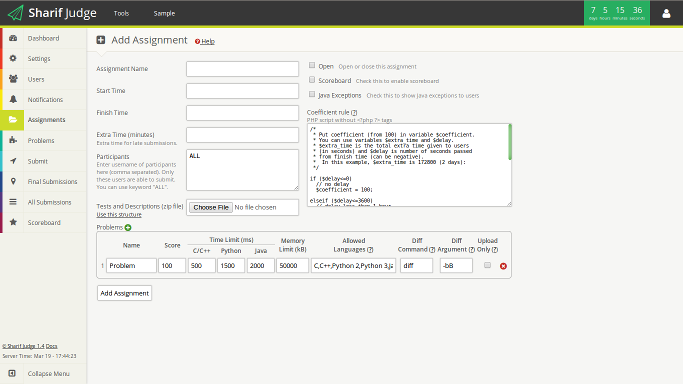
\includegraphics[width=1.0\textwidth]{add_assignment}  
			\caption[Tampilan Halaman \textit{Assignments}]{Tampilan Halaman \textit{Assignments}} 
			\label{fig:add_assignment} 
		\end{figure} 
		
		Berikut ini adalah pengaturan yang terdapat pada halaman \textit{Add Assignments}:
		\begin{itemize}
			\item \textit{Assignment Name} \\
			Nama \textit{assignment} yang akan ditampilkan dalam daftar \textit{assignment}.
			
			\item \textit{Start Time} \\
			\textit{User} tidak dapat mengumpulkan assignment sebelum \textit{"Start Time"}. Format yang digunakan untuk pengaturan start time adalah \textit{MM/DD/YYYY HH:MM:SS}. Contohnya: 08/31/2013 12:00:00
			
			\item \textit{Finish Time, Extra Time} \\
			Peserta tidak dapat mengumpulkan \textit{assignment} setelah \textit{Finish Time + Extra Time}. \textit{Assignment} yang telat akan dikalikan dengan koefisien tertentu. Pengguna harus menulis \textit{script} PHP untuk menghitung koefisien pada bidang \textit{"Coefficient Rule"}. Format yang digunakan untuk pengaturan \textit{finish time} adalah \textit{MM/DD/YYYY HH:MM:SS}. Contoh: \textit{08/31/2013 23:59:59}. "\textit{Extra Time}" akan terhitung dalam satuan menit. Pengguna juga dapat menggunakan operator aritmatika seperti *, -, +, /. Contohnya \textit{120} (2 jam) atau \textit{48*60} (2 hari).
			
			\item \textit{Participants} \\
			Pengguna dapat menggunakan kata kunci \textit{ALL} pada kolom \textit{Participants} untuk mengijinkan seluruh peserta agar dapat mengumpulkan \textit{assignment}. Untuk membatasi peserta tertentu, pengguna dapat memasukan \textit{username} peserta pada kolom \textit{Participants}. Setiap \textit{username} dapat dipisahkan menggunakan tanda koma. Contoh: \textit{admin, instructor1, instructor2, student1, student2, student3, student4}.
			
			\item \textit{Test} \\
			Pengguna dapat mengunggah \textit{test cases} dalam bentuk \textit{zip file} dengan struktur yang sudah ditentukan.
			
			\item \textit{Open} \\
			Pengguna dapat membuka atau menutup \textit{assignment} untuk \textit{user students} menggunakan pilihan ini. Jika pengguna menutup \textit{assignment}, \textit{non-student users} masih dapat mengumpulkan \textit{assignment}.
			
			\item \textit{Scoreboard} \\
			Pengguna dapat mengaktifkan atau menonaktifkan papan nilai dengan menggunakan pilihan ini.
			
			\item \textit{Java Exceptions} \\
			Pengguna dapat mengaktifkan dan menonaktifkan \textit{java exception} yang ditunjukan kepada \textit{students}. Perubahan pada pilihan ini tidak memengaruhi kode yang sebelumnya sudah dinilai. Nama \textit{exception} akan muncul jika pada \textit{file} path{tester/java\_exceptions\_list} berisikan nama \textit{exception} tersebut. Berikut adalah hasil \textit{exception} yang ditunjukan jika pengguna mengaktifkan pengaturan \textit{Java Exceptions}: \\
			
			\begin{lstlisting}[basicstyle=\ttfamily, frame=single,
			columns=fullflexible, keepspaces=true, breaklines=true, label=ls:6]
Test 1
ACCEPT
Test 2
Runtime Error (java.lang.ArrayIndexOutOfBoundsException)
Test 3
Runtime Error (java.lang.ArrayIndexOutOfBoundsException)
Test 4
ACCEPT
Test 5
ACCEPT
Test 6
ACCEPT
Test 7
ACCEPT
Test 8
Runtime Error (java.lang.ArrayIndexOutOfBoundsException)
Test 9
Runtime Error (java.lang.StackOverflowError)
Test 10
Runtime Error (java.lang.ArrayIndexOutOfBoundsException)
			\end{lstlisting}
			
			\item \textit{Archieved Assignment} \\
			Jika fitur ini diaktifkan maka \textit{assignment} akan dibuat dengan \textit{Finish Time} 2038-01-18 00:00:00 (\textit{UTC}+ 7) dalam kata lain pengguna memiliki waktu yang tidak terbatas untuk mengumpulkan \textit{assignment} tersebut.
			
			\item \textit{Coefficient Rule} \\
			Pengguna dapat menulis \textit{script} PHP pada bagian ini. Pengguna harus memasukan koefisien (dari 100) pada variabel \textit{\$coefficient}. Pengguna dapat menggunakan variabel \textit{\$extra\_time} dan \textit{\$delay}. \textit{\$extra\_time} merupakan total waktu ekstra yang diberikan kepada \textit{users} dalam satuan detik dan \textit{\$delay} merupakan jumlah detik berlalu dari waktu selesai (dapat negatif). \textit{Script} PHP pada bagian ini tidak boleh mengandung \textit{tags <?php , <? , ?>}. Berikut contoh \textit{\$extra\_time} 172800 (2 hari):
			
			\begin{lstlisting}[basicstyle=\ttfamily, frame=single,
			columns=fullflexible, keepspaces=true, breaklines=true, label=ls:7]
if ($delay<=0)
// no delay
$coefficient = 100;

elseif ($delay<=3600)
// delay less than 1 hour
$coefficient = ceil(100-((30*$delay)/3600));

elseif ($delay<=86400)
// delay more than 1 hour and less than 1 day
$coefficient = 70;

elseif (($delay-86400)<=3600)
// delay less than 1 hour in second day
$coefficient = ceil(70-((20*($delay-86400))/3600));

elseif (($delay-86400)<=86400)
// delay more than 1 hour in second day
$coefficient = 50;

elseif ($delay > $extra_time)
// too late
$coefficient = 0;
			\end{lstlisting}
			
			\item \textit{Time Limit} \\
			Pengguna dapat mengatur batas waktu untuk menjalankan kode dalam satuan milisekon. Program yang ditulis menggunakan \textit{Python} dan \textit{Java} biasanya lebih lambat dari \textit{C/C++}. Oleh karena itu \textit{Python} dan \textit{Java} membutuhkan waktu yang lebih.
			
			\item \textit{Memory Limit} \\
			Pengguna dapat mengatur batas memori dalam satuan \textit{kilobytes}, namun penggunaan \textit{Memory Limit} tidak terlalu akurat.
			
			\item \textit{Allowed Languages} \\
			Pengguna dapat mengatur bahasa untuk setiap \textit{problem} (dipisahkan menggunakan koma). Bahasa yang tersedia seperti \textit{C, C++, Java, Python 2, Python 3, zip, PDF}. Pengguna dapat menggunakan \textit{zip} atau \textit{PDF} jika mengaktifkan pilihan \textit{Upload Only}. Contoh: \textit{C, C++ , zip} atau \textit{Python 2,Python 3} atau \textit{Java ,C}.
			
			\item \textit{Diff Command} \\
			\textit{Command} ini digunakan untuk membandingkan keluaran dengan keluaran yang benar. Secara standar \textit{SharIF Judge} menggunakan \textit{diff}, namun pengguna dapat mengubah \textit{command} pada bagian ini. Bidang ini tidak boleh mengandung spasi.
			
			\item \textit{Diff Arguments} \\
			Pengguna dapat mengatur argumen dari \textit{Diff Command} disini. Pengguna dapat melihat \textit{man diff} untuk melihat daftar lengkap \textit{diff} argumen. \textit{SharIF Judge} menambahkan dua pilihan baru yaitu \textit{ignore} dan \textit{identical}. \textit{Ignore} akan menghiraukan semua baris baru dan spasi. \textit{Identical} tidak akan menghiraukan apapun namun keluaran dari file yang dikumpulkan harus identik dengan keluaran \textit{test case} agar dapat diterima.
			
			\item \textit{Upload Only} \\
			Jika pengguna mengatur \textit{problem} sebagai \textit{Upload-Only}, maka \textit{SharIF Judge} tidak akan menilai \textit{assignment} pada \textit{problem} tersebut. Pengguna dapat menggunakan \textit{zip} dan \textit{PDF} pada \textit{allowed languages} jika mengaktifkan pilihan ini.
			
		\end{itemize}
		
		\subsection*{\textit{Sample Assignment}}
		\label{subsec:sample_assignment}
		Berikut adalah contoh \textit{assignment} untuk testing pada \textit{SharIF Judge}. Untuk menambah \textit{assignment} pengguna dapat menekan \textit{Add} pada halaman \textit{Assignments}.
		
		\begin{enumerate}
			\item \textit{Problem} 1 (Penjumlahan) \\
			Program pengguna akan menerima bilangan integer n, kemudian menerima masukkan sebanyak n buah bilangan integer dan akan menampilkan hasil penjumlahan n buah bilangan integer tersebut. Tabel \ref{tab:problem_sum} menunjukkan contoh hasil masukkan dan keluaran \textit{problem 1}.
			
			\begin{table}[H]
				\centering 
				\caption{\textit{Problem} 1 (Penjumlahan)}
				\label{tab:problem_sum}
				\begin{tabular}{|c|c|}
					\hline
					Sample Input & Sample Output\\
					
					\hline
					\multicolumn{1}{|l|}{5} & \multirow{2}{*}{145}\\
					\multicolumn{1}{|l|}{54 78 0 4 9} & \\
					
					\hline
					
				\end{tabular} 
			\end{table}
			
			\item \textit{Problem} 2 (\textit{Max}) \\
			Program pengguna akan menerima bilangan integer n, kemudian menerima masukkan sebanyak n buah bilangan integer dan akan menampilkan hasil penjumlahan dari dua nilai tertinggi. Tabel \ref{tab:problem_max} menunjukkan contoh hasil masukkan dan keluaran \textit{problem 2}.
			
			\begin{table}[H]
				\centering 
				\caption{\textit{Problem} 2 (\textit{Max})}
				\label{tab:problem_max}
				\begin{tabular}{|c|c|}
					\hline
					Sample Input & Sample Output\\
					
					\hline
					\multicolumn{1}{|l|}{7} & \multirow{2}{*}{356}\\
					\multicolumn{1}{|l|}{162 173 159 164 181 158 175} & \\
					
					\hline
					
				\end{tabular} 
			\end{table}
			
			\item \textit{Problem} 3 \textit{Upload} \\
			Program pengguna akan menerima sebuah \textit{file C} atau \textit{zip}. \textit{Problem} ini menggunakan pilihan \textit{Upload Only} sehingga tidak dinilai oleh \textit{SharIF Judge}.
		\end{enumerate}
		
		Pengguna dapat menemukan \textit{file zip} pada folder \textit{Assignment}. Berikut susunan pohon dari tiga \textit{problem} di atas:
		
		\begin{lstlisting}[basicstyle=\ttfamily, frame=single,
		columns=fullflexible, keepspaces=true, breaklines=true, label=ls:8]
.
|-- p1
|   |-- in
|   |   |-- input1.txt
|   |   |-- input2.txt
|   |   |-- input3.txt
|   |   |-- input4.txt
|   |   |-- input5.txt
|   |   |-- input6.txt
|   |   |-- input7.txt
|   |   |-- input8.txt
|   |   |-- input9.txt
|   |   --- input10.txt
|   |-- out
|   |   --- output1.txt
|   |-- tester.cpp
|   --- desc.md
|-- p2
|   |-- in
|   |   |-- input1.txt
|   |   |-- input2.txt
|   |   |-- input3.txt
|   |   |-- input4.txt
|   |   |-- input5.txt
|   |   |-- input6.txt
|   |   |-- input7.txt
|   |   |-- input8.txt
|   |   |-- input9.txt
|   |   --- input10.txt
|   |-- out
|   |   |-- output1.txt
|   |   |-- output2.txt
|   |   |-- output3.txt
|   |   |-- output4.txt
|   |   |-- output5.txt
|   |   |-- output6.txt
|   |   |-- output7.txt
|   |   |-- output8.txt
|   |   |-- output9.txt
|   |   --- output10.txt
|   |-- desc.md
|   --- Problem2.pdf
|-- p3
|   --- desc.md
--- SampleAssignment.pdf
		\end{lstlisting}
		
		\textit{Problem} 1 menggunakan metode \textit{"Tester"} untuk memeriksa keluaran, sehingga memiliki \textit{file tester.cpp (Tester Script)}. \textit{Problem} 2 menggunakan metode \textit{Output Comparison} untuk memeriksa keluaran, sehingga memiliki dua folder (\textit{in} dan \textit{out}) yang berisi \textit{test case}. \textit{Problem} 3 menggunakan pilihan \textit{Upload-Only}.
		
		\subsection*{\textit{Test Structure}}
		\label{subsec:test_structure}
		Saat menambah \textit{assignments}, pengguna harus menyediakan \textit{file zip} yang berisi \textit{test cases}. \textit{File zip} ini berisi folder-folder untuk setiap \textit{problem}. Pengguna harus memberi nama folder sesuai aturan seperti \textit{p1, p2, p3}, dst. \textit{Assignment} yang menggunakan pilihan \textit{Upload-Only} tidak membutuhkan \textit{folder}.
		
		\subsubsection*{Metode Pengecekan}
		\label{subsubsec:metode_pengecekan}
		\textit{SharIF Judge} memiliki dua metode pengecekan untuk setiap \textit{problem} yaitu metode \textit{"Input/Output Comparison"} dan metode \textit{"Tester"}.
		
		\begin{enumerate}
			\item Metode \textit{Input/Output Comparison} \\
			Dalam metode ini pengguna harus memasukkan beberapa \textit{file input} dan beberapa \textit{output} ke dalam folder \textit{problem}. \textit{SharIF Judge} akan memasukkan nilai dari \textit{file input} ke kode \textit{users} dan membandingkan hasil keluaran dari kode \textit{users} dengan \textit{file output}. \textit{Input files} harus berada dalam folder \textit{"in"} dengan nama \textit{input1.txt, input2.txt,} dst. \textit{Output files} harus berada dalam folder \textit{"out"} dengan nama \textit{output1.txt, output2.txt,} dst.
			
			\item Metode \textit{Tester} \\
			Dalam metode ini pengguna harus memasukkan beberapa \textit{file input}, sebuah \textit{file C++ (tester.cpp)}, dan beberapa \textit{file output}. \textit{SharIF Judge} akan memasukkan nilai dari \textit{file input} ke kode \textit{users} dan mengambil keluaran dari kode \textit{users}. \textit{tester.cpp} akan mengambil nilai dari \textit{file input, file output,} dan keluaran \textit{users}. Jika keluaran dari kode \textit{users} benar maka akan mengembalikan nilai 0, sedangkan jika salah akan mengembalikan nilai 1.
			
			Pengguna dapat menggunakan kode pada listing \ref{ls:9} sebagai templat untuk menulis \textit{tester.cpp}:
			\begin{lstlisting}[basicstyle=\ttfamily, frame=single,
			columns=fullflexible, keepspaces=true, breaklines=true, label=ls:9, caption=Contoh kode \textit{tester.cpp}]
/*
* tester.cpp
*/

#include <iostream>
#include <fstream>
#include <string>
using namespace std;
int main(int argc, char const *argv[])
{

ifstream test_in(argv[1]);    /* This stream reads from test's input file   */
ifstream test_out(argv[2]);   /* This stream reads from test's output file  */
ifstream user_out(argv[3]);   /* This stream reads from user's output file  */

/* Your code here */
/* If user's output is correct, return 0, otherwise return 1       */

...

			}
			\end{lstlisting}
		\end{enumerate}
		
		\subsubsection*{Contoh \textit{File}}
		\label{subsubsec:contoh_file}
		Pengguna dapat menemukan contoh \textit{file} penguji dalam folder \textit{Assignments}. Berikut contoh susunan pohon dari \textit{file} tersebut:
		
		\begin{lstlisting}[basicstyle=\ttfamily, frame=single,
		columns=fullflexible, keepspaces=true, breaklines=true, label=ls:10]
.
|-- p1
|   |-- in
|   |   |-- input1.txt
|   |   |-- input2.txt
|   |   |-- input3.txt
|   |   |-- input4.txt
|   |   |-- input5.txt
|   |   |-- input6.txt
|   |   |-- input7.txt
|   |   |-- input8.txt
|   |   |-- input9.txt
|   |   --- input10.txt
|   |-- out
|   |   --- output1.txt
|   --- tester.cpp
--- p2
|-- in
|   |-- input1.txt
|   |-- input2.txt
|   |-- input3.txt
|   |-- input4.txt
|   |-- input5.txt
|   |-- input6.txt
|   |-- input7.txt
|   |-- input8.txt
|   |-- input9.txt
|   --- input10.txt
--- out
|-- output1.txt
|-- output2.txt
|-- output3.txt
|-- output4.txt
|-- output5.txt
|-- output6.txt
|-- output7.txt
|-- output8.txt
|-- output9.txt
--- output10.txt
		\end{lstlisting}
		
		\textit{Problem} 1 menggunakan metode \textit{"Tester"} untuk mengecek hasil keluarannya sehingga memiliki \textit{file tester.cpp}. Listing \ref{ls:11} menunjukkan isi dari \textit{file tester.cpp} untuk \textit{Problem} 1:
		
		\begin{lstlisting}[basicstyle=\ttfamily, frame=single,
		columns=fullflexible, keepspaces=true, breaklines=true, label=ls:11, caption=Isi \textit{File tester.cpp} untuk \textit{Problem} 1]
/*
* tester.cpp
*/

#include <iostream>
#include <fstream>
#include <string>
using namespace std;
int main(int argc, char const *argv[])
{

	ifstream test_in(argv[1]);    /* This stream reads from test's input file   */
	ifstream test_out(argv[2]);   /* This stream reads from test's output file  */
	ifstream user_out(argv[3]);   /* This stream reads from user's output file  */
	
	/* Your code here */
	/* If user's output is correct, return 0, otherwise return 1       */
	/* e.g.: Here the problem is: read n numbers and print their sum:  */
	
	int sum, user_output;
	user_out >> user_output;
	
	if ( test_out.good() ) // if test's output file exists
	{
		test_out >> sum;
	}
	else
	{
		int n, a;
		sum=0;
		test_in >> n;
		for (int i=0 ; i<n ; i++){
			test_in >> a;
			sum += a;
		}
	}

	if (sum == user_output)
		return 0;
	else
		return 1;

}
		\end{lstlisting}
		
		\textit{Problem} 2 menggunakan metode \textit{"Input/Output Comparison"} untuk mengecek hasil keluarannya sehingga memiliki dua folder \textit{in} dan \textit{out} yang berisi \textit{test cases}. \textit{Problem} 3 menggunakan pilihan \textit{Upload-Only} sehingga tidak memiliki folder apapun.
		
		\subsection*{Deteksi Kecurangan}
		\label{subsec:deteksi_kecurangan}
		\textit{SharIF Judge} menggunakan \textit{Moss} untuk mendeteksi kode yang mirip. \textit{Moss (Measure Of Software Similarity)} merupakan sistem otomatis untuk menentukan kemiripan program. Pada saat ini, aplikasi utama \textit{Moss} telah digunakan untuk mendeteksi plagiarisme pada kelas \textit{programming}. Pengguna dapat mengirimkan kode final (yang dipilih oleh \textit{students} sebagai \textit{Final Submission}) ke server \textit{Moss} dengan satu klik.
		
		Sebelum menggunakan \textit{Moss} ada beberapa hal yang perlu diperhatikan yaitu:
		
		\begin{itemize}
			\item Pengguna harus mendapatkan \textit{Moss user id} dan mengaturnya di \textit{SharIF Judge}. Untuk mendapatkan \textit{Moss user id}, pengguna harus terlebih dahulu mendaftar pada halaman \path{http://theory.stanford.edu/~aiken/moss/}. Pengguna akan menerima sebuah \textit{email} yang berisi \textit{script perl}. Dalam \textit{script} tersebut terdapat \textit{Moss user id}.
			
			Listing \ref{ls:12} menunjukkan potongan \textit{script perl} yang mengandung \textit{user id}:
			\begin{lstlisting}[basicstyle=\ttfamily, frame=single,
			columns=fullflexible, keepspaces=true, breaklines=true, label=ls:12, caption=Potongan \textit{script perl}]
...

$server = 'moss.stanford.edu';
$port = '7690';
$noreq = "Request not sent.";
$usage = "usage: moss [-x] [-l language] [-d] 
[-b basefile1] ... [-b basefilen] [-m #] 
[-c \"string\"] file1 file2 file3 ...";

#
# The userid is used to authenticate your queries to the server; 
don't change it!
#
$userid=YOUR_MOSS_USER_ID;

#
# Process the command line options.  This is done in a non-standard
# way to allow multiple -b's.
#
$opt_l = "c";   # default language is c
$opt_m = 10;
$opt_d = 0;

...
			}
			
			\end{lstlisting}
			
			\textit{User id} yang terdapat pada potongan \textit{script perl} di atas, dapat digunakan pada \textit{SharIF Judge} pada halaman \textit{Moss}. \textit{SharIF Judge} akan menggunakan \textit{user id} tersebut di \textit{Moss perl script}. \textit{Perl} harus terinstal pada server agar dapat menggunakan \textit{Moss}.  
			
			\item Pengguna dianjurkan untuk mendeteksi kode yang mirip setelah waktu \textit{assignment} selesai, karena para peserta masih dapat mengubah \textit{Final Submissions} masing-masing sebelum waktu habis. Dengan cara tersebut, \textit{SharIF Judge} dapat mengirimkan \textit{Final submissions} para peserta ke \textit{server Moss}.
		\end{itemize}
		
		\subsection*{Keamanan}
		\label{subsec:keamanan}
		Pengguna dapat mengatur keamanan \textit{SharIF Judge} dengan beberapa langkah. Berikut adalah langkah-langkah yang dapat dilakukan.
		
		\subsubsection*{Memakai \textit{Sandbox}}
		\label{subsubsec:memakai_sandbox}
		Pengguna harus memakai \textit{Sandbox} untuk \textit{C/C++} dan mengaktifkan \textit{Java Security Manager (Java Policy)} untuk \textit{Java}. Penjelasan lebih lanjut tentang \textit{Sandbox} ada pada point \ref{subsec:sandbox}.
		
		\subsubsection*{Memakai \textit{Shield}}
		\label{subsubsec:memakai_shield}
		\textit{Shield} bukan merupakan pertahanan yang asli, tetapi lebih baik ada daripada tidak sama sekali. Pengguna dapat mengaktifkan \textit{Shield} untuk \textit{C, C++, Python}. Penjelasan lebih lanjut tentang \textit{Shield} ada pada point \ref{subsubsec:shield}.
		
		\subsubsection*{Jalankan sebagai \textit{Non-Privileged User}}
		\label{subsubsec:non_prileged_user}
		Pengguna diharapkan menjalankan kode yang sudah dikumpulkan sebagai \textit{non-privileged user} - \textit{user} yang tidak memiliki akses jaringan, tidak dapat menulis \textit{file} apapun, dan tidak dapat membuat banyak proses.
		
		Pengguna harus menjalankan \textit{PHP} pada server sebagai \textit{user www-data}. Membuat \textit{user} baru dengan nama \textit{restricted\_user} dan passwordnya. Jalankan \textit{sudo visudo} dan tambahkan baris berikut pada akhir file \textit{sudoers} :
		
		\begin{lstlisting}[basicstyle=\ttfamily, frame=single,
		columns=fullflexible, keepspaces=true, breaklines=true, label=ls:13]
www-data ALL=(restricted_user) NOPASSWD: ALL
		\end{lstlisting}
		
		Pada file \textit{tester/runcode.sh} ganti 
		
		\begin{lstlisting}[basicstyle=\ttfamily, frame=single,
		columns=fullflexible, keepspaces=true, breaklines=true, label=ls:14]
if $TIMEOUT_EXISTS; then
	timeout -s9 $((TIMELIMITINT*2)) $CMD <$IN >out 2>err
else
	$CMD <$IN >out 2>err        
fi
		\end{lstlisting}
		
		menjadi
		
		\begin{lstlisting}[basicstyle=\ttfamily, frame=single,
		columns=fullflexible, keepspaces=true, breaklines=true, label=ls:15]
if $TIMEOUT_EXISTS; then
	sudo -u restricted_user timeout -s9 $((TIMELIMITINT*2)) $CMD <$IN >out 2>err
else
	sudo -u restricted_user $CMD <$IN >out 2>err        
fi
		\end{lstlisting}
		
		dan \textit{uncomment} baris berikut:
		
		\begin{lstlisting}[basicstyle=\ttfamily, frame=single,
		columns=fullflexible, keepspaces=true, breaklines=true, label=ls:16]
sudo -u restricted_user pkill -9 -u restricted_user
		\end{lstlisting}
		
		\begin{itemize}
			\item Menonaktifkan jaringan pada \textit{restricted\_user} \\
			\textit{restricted\_user} seharusnya tidak dapat mengakses jaringan. Pengguna dapat menonaktifkan jaringan untuk sebuah \textit{user} pada \textit{Linux} dengan menggunakan \textit{iptables}. Setelah dinonaktifkan, uji dengan \textit{ping} sebagai \textit{restricted\_user}.
			
			\item Menolak izin menulis \\
			Pastikan tidak ada \textit{file} atau \textit{directory} yang dapat ditulis oleh \textit{restricted\_user}.
			
			\item Membatasi jumlah proses \\
			Pengguna dapat membatasi jumlah proses dengan cara menambahkan baris berikut pada file \textit{/etc/security/limits.conf}:
			
			\begin{lstlisting}[basicstyle=\ttfamily, frame=single,
			columns=fullflexible, keepspaces=true, breaklines=true, label=ls:17]
restricted_user     soft    nproc   3
restricted_user     hard    nproc   5
			\end{lstlisting}
			
		\end{itemize}
		
		\subsubsection*{Memakai Dua \textit{Server}}
		\label{subsubsec:memakai_dua_server}
		Pengguna dapat memakai sebuah \textit{server} untuk antarmuka web dan menangani permintaan web, dan memakai \textit{server} lainnya untuk menjalankan kode yang dikumpulkan. Hal ini mengurangi risiko menjalankan kode yang dikumpulkan. Untuk memakai dua \textit{server} pengguna harus mengganti \textit{source code SharIF Judge}. 
		
		
		\subsection*{\textit{Sandbox}}
		\label{subsec:sandbox}
		\textit{SharIF Judge} menjalankan banyak \textit{arbitary codes} yang \textit{user} kumpulkan sehingga memerlukan perkakas untuk kode \textit{sandbox} yang sudah dikumpulkan. Pengguna dapat meningkatkan keamanan dengan cara mengaktifkan \textit{shield} dan \textit{sandbox} secara bersamaan.
		
		\subsubsection*{\textit{C/C++ Sandboxing}}
		\label{subsubsec:sandbox_c/c++}
		\textit{SharIF Judge} menggunakan \textit{EasySandbox} untuk \textit{sandboxing} kode \textit{C/C++}. \textit{EasySandbox} membatasi jalannya kode mengguna \textit{seccomp}, mekanisme \textit{sandboxing} pada \textit{Linux kernel}.
		
		Secara standar, \textit{EasySandbox} dinonaktifkan pada \textit{SharIF Judge}. Pengguna dapat mengaktifkannya pada halaman \textit{Settings}. Pengguna harus \textit{"Build EasySandbox"} sebelum mengaktifkannya.
		
		\paragraph{Build EasySandbox}
		\textit{EasySandbox files} terletak pada \textit{tester/easysandbox}. Untuk membangun \textit{EasySandbox} jalankan :
		
		\begin{lstlisting}[basicstyle=\ttfamily, frame=single,
		columns=fullflexible, keepspaces=true, breaklines=true, label=ls:18]
$ cd tester/easysandbox
$ chmod +x runalltests.sh
$ chmod +x runtest.sh
$ make runtests
		\end{lstlisting}
		
		Jika pesan yang ditampilkan adalah \textit{"All tests passed!"}, maka \textit{EasySandbox} telah berhasil dibangun dan dapat dipakai pada sistem. Pengguna dapat mengaktifkan \textit{EasySandbox} pada halaman \textit{Settings}.
		
		\subsubsection*{\textit{Java Sandboxing}}
		\label{subsubsec:java_sandbox}
		\textit{Java Sandbox} dapat diaktifkan secara standar menggunakan \textit{Java Security Manager}. Pengguna dapat mengaktifkan/menonaktifkan hal ini pada halaman \textit{Settings}.
		
		\subsection*{\textit{Shield}}
		\label{subsubsec:shield}
		\textit{Shield} merupakan mekanisme sederhana yang melarang jalannya kode yang berbahaya. \textit{Shield} bukan solusi \textit{sandboxing}. \textit{Shield} hanya menyediakan sebagian pertahanan terhadap serangan sepele. Pertahanan yang asli terhadap kode yang tidak terpercaya hanya didapatkan dengan mengaktifkan \textit{Sandbox}.
		
		\subsubsection*{\textit{Shield} untuk \textit{C/C++}}
		\label{subsubsec:shield_c/c++}
		Dengan mengaktifkan \textit{Shield} untuk \textit{C/C++}, \textit{SharIF Judge} hanya menambahkan \textit{\#define} pada bagian awal kode \textit{C/C++} sebelum menjalankannya.
		
		Pengguna dapat melarang menggunakan \textit{goto} dengan cara menambahkan baris berikut pada bagian awal kode yang dikumpulkan :
		
		\begin{lstlisting}[basicstyle=\ttfamily, frame=single,
		columns=fullflexible, keepspaces=true, breaklines=true, label=ls:19]
#define goto YouCannotUseGoto
		\end{lstlisting}
		
		Dengan baris ini pada awal \textit{files}, semua kode yang sudah dikumpulkan yang menggunakan \textit{goto} akan mendapatkan \textit{compilation error}.
		
		Jika pengguna menggunakan \textit{Shield}, semua kode yang berisi \textit{\#undef} akan mendapatkan \textit{compilation error}.
		
		\subsubsection*{Mengaktifkan \textit{Shield} untuk \textit{C} atau \textit{C++}}
		\label{subsubsec:mengaktifkan_shield_c/c++}
		Pengguna dapat mengaftikan dan menonaktifkan \textit{Shield} pada halaman \textit{Settings}.
		
		\subsubsection*{Menambahkan aturan untuk \textit{C/C++}}
		\label{subsubsec:menambah_aturan_c/c++}
		Daftar aturan \textit{\#define} terletak pada \textit{file} \textit{tester/shield/defc.h} (untuk \textit{C}) dan \textit{tester/shield/defcpp.h} (untuk \textit{C++}). Pengguna dapat menambahkan aturan \textit{\#define} baru pada \textit{file} ini. Konten dari \textit{file} ini dapat diganti pada halaman \textit{Settings}.
		
		Berikut adalah sintaksis yang digunakan pada \textit{files} tersebut :
		
		\begin{lstlisting}[basicstyle=\ttfamily, frame=single,
		columns=fullflexible, keepspaces=true, breaklines=true, label=ls:20]
/*

@file defc.h
There should be a newline at end of this file.
Put the message displayed to user after // in each line

e.g. If you want to disallow goto, add this line:
#define goto errorNo13    //Goto is not allowd

*/

#define system errorNo1      //"system" is not allowed
#define freopen errorNo2     //File operation is not allowed
#define fopen errorNo3       //File operation is not allowed
#define fprintf errorNo4     //File operation is not allowed
#define fscanf errorNo5      //File operation is not allowed
#define feof errorNo6        //File operation is not allowed
#define fclose errorNo7      //File operation is not allowed
#define ifstream errorNo8    //File operation is not allowed
#define ofstream errorNo9    //File operation is not allowed
#define fork errorNo10       //Fork is not allowed
#define clone errorNo11      //Clone is not allowed
#define sleep errorNo12      //Sleep is not allowed
		\end{lstlisting}
		
		Pada akhir \textit{files} \textit{defc.h} dan \textit{defcpp.h} harus ada baris baru. Ada banyak aturan yang tidak dapat dipakai pada \textit{g++}. Sebagai contoh pengguna tidak dapat memakai \textit{\#define fopen errorNo3} pada \textit{C++} karena hasilnya \textit{compile error}.
		
		\subsubsection*{\textit{Shield} untuk \textit{Python}}
		\label{subsubsec:shield_python}
		Dengan mengaktifkan \textit{Shield} untuk \textit{Python}, \textit{SharIF Judge} hanya menambahkan beberapa kode pada bagian awal kode \textit{Python} yang telah dikumpulkan sebelum dijalankan untuk mencegah penggunaan fungsi yang berbahaya. Kode tersebut terletak pada \textit{files} \textit{tester/shield/shield\_py2.py} dan \textit{tester/shield/shield\_py3.py}. Pengguna dapat mengaktifkan/menonaktifkan \textit{Shield} untuk \textit{Python} pada halaman \textit{Settings}.
		
		Berikut adalah cara untuk keluar dari \textit{Shield} dan menggunakan fungsi yang telah di \textit{blacklist} :
		
		\begin{lstlisting}[basicstyle=\ttfamily, frame=single,
		columns=fullflexible, keepspaces=true, breaklines=true, label=ls:21]
# @file shield_py3.py

import sys
sys.modules['os']=None

BLACKLIST = [
#'__import__', # deny importing modules
'eval', # eval is evil
'open',
'file',
'exec',
'execfile',
'compile',
'reload',
#'input'
]
for func in BLACKLIST:
if func in __builtins__.__dict__:
del __builtins__.__dict__[func]
		\end{lstlisting}
		
		
		\item \textbf{Mengukur tingkat kepatuhan aplikasi \textit{SharIF Judge} terhadap \textit{WCAG 2.1}}\\
		{\bf Status :} Ada sejak rencana kerja skripsi.\\
		{\bf Hasil :} Kesuksesan aplikasi \textit{SharIF Judge} dalam mematuhi kriteria sukses \textit{WCAG} 2.1 ditulis dalam tabel-tabel berikut.
		
		\begin{table}[H]
			\centering
			\caption{Tabel kepatuhan \textit{SharIF Judge} terhadap prinsip \textit{Perceivable}}
			\label{tab:kepatuhan_sharif_judge_perceivable}
			\begin{tabular}{|c|c|c|}
				\hline
				Kriteria Sukses & Tingkat Kepatuhan & Hasil \\
				\hline
				1.1.1 & Tidak Sukses & A\\
				1.2.1 & Sukses & A\\
				1.2.2 & Sukses & A\\
				1.2.3 & Sukses & A\\
				1.2.4 & Sukses & AA\\
				1.2.5 & Sukses & AA\\
				1.2.6 & Sukses & AAA\\
				1.2.7 & Sukses & AAA\\
				1.2.8 & Sukses & AAA\\
				1.2.9 & Sukses & AAA\\
				1.3.1 & Tidak Sukses & A\\
				1.3.2 & Sukses & A\\
				1.3.3 & Sukses & A\\
				1.3.4 & Sukses & A\\
				1.3.5 & Tidak Sukses & AA \\
				1.3.6 & Tidak Sukses & AAA \\
				1.4.1 & Sukses & A\\
				1.4.2 & Sukses & A\\
				1.4.3 & Tidak Sukses & AA\\
				1.4.4 & Tidak Sukses & AA\\
				1.4.5 & Sukses & AA\\
				1.4.6 & Tidak Sukses & AAA\\
				1.4.7 & Sukses & AAA\\
				1.4.8 & Tidak Sukses & AAA\\
				1.4.9 & Sukses & AAA\\
				1.4.10 & Tidak Sukses & AA \\
				1.4.11 & Diabaikan & AA \\
				1.4.12 & Sukses & AA\\
				1.4.13 & Sukses & AA\\
				\hline
				\multicolumn{2}{|c|}{Kesimpulan} & - \\
				\hline
			\end{tabular}
		\end{table}
		
		\begin{table}[H]
			\centering
			\caption{Tabel kepatuhan \textit{SharIF Judge} terhadap prinsip \textit{Operable}}
			\label{tab:kepatuhan_sharif_judge_operable}
			\begin{tabular}{|c|c|c|}
				\hline
				Kriteria Sukses & Tingkat Kepatuhan & Hasil \\
				\hline
				2.1.1 & Tidak Sukses & A\\
				2.1.2 & Tidak Sukses & A\\
				2.1.3 & Tidak Sukses & AAA\\
				2.1.4 & Sukses & A\\
				2.2.1 & Sukses & A\\
				2.2.2 & Sukses & A\\
				2.2.3 & Sukses & AAA\\
				2.2.4 & Sukses & AAA\\
				2.2.5 & Tidak Sukses & AAA\\
				2.2.6 & Tidak Sukses & AAA\\
				2.3.1 & Sukses & A\\
				2.3.2 & Sukses & AAA\\
				2.3.3 & Sukses & AAA\\
				2.4.1 & Tidak Sukses & A\\
				2.4.2 & Sukses & A\\
				2.4.3 & Sukses & AA\\
				2.4.4 & Tidak Sukses & A\\
				2.4.5 & Tidak Sukses & AA\\
				2.4.6 & Tidak Sukses & AA\\
				2.4.7 & Tidak Sukses & AA\\
				2.4.8 & Sukses & AAA\\
				2.4.9 & Tidak Sukses & AAA\\
				2.4.10 & Tidak Sukses & AAA\\
				2.5.1 & Sukses & A\\
				2.5.2 & Sukses & A\\
				2.5.3 & Tidak Sukses & A\\
				2.5.4 & Sukses & A\\
				2.5.5 & Tidak Sukses & AAA\\
				2.5.6 & Sukses & AAA\\
				\hline
				\multicolumn{2}{|c|}{Kesimpulan} & - \\
				\hline
			\end{tabular}
		\end{table}
		
		\begin{table}[H]
			\centering
			\caption{Tabel kepatuhan \textit{SharIF Judge} terhadap prinsip \textit{Understandable}}
			\label{tab:kepatuhan_sharif_judge_understandable}
			\begin{tabular}{|c|c|c|}
				\hline
				Kriteria Sukses & Tingkat Kepatuhan & Hasil \\
				\hline
				3.1.1 & Tidak Sukses & A\\
				3.1.2 & Tidak Sukses & AA\\
				3.1.3 & Sukses & AAA\\
				3.1.4 & Sukses & AAA\\
				3.1.5 & Sukses & AAA\\
				3.1.6 & Sukses & AAA\\
				3.2.1 & Sukses & A\\
				3.2.2 & Sukses & A\\
				3.2.3 & Sukses & AA\\
				3.2.4 & Tidak Sukses & AA\\
				3.2.5 & Sukses & AAA\\
				3.3.1 & Sukses & A\\
				3.3.2 & Tidak Sukses & A\\
				3.3.3 & Sukses & AA\\
				3.3.4 & Sukses & AA\\
				3.3.5 & Tidak Sukses & AAA\\
				3.3.6 & Sukses & AAA\\
				\hline
				\multicolumn{2}{|c|}{Kesimpulan} & - \\
				\hline
			\end{tabular}
		\end{table}
		
		\begin{table}[H]
			\centering
			\caption{Tabel kepatuhan \textit{SharIF Judge} terhadap prinsip \textit{Robust}}
			\label{tab:kepatuhan_sharif_judge_robust}
			\begin{tabular}{|c|c|c|}
				\hline
				Kriteria Sukses & Tingkat Kepatuhan & Hasil \\
				\hline
				4.1.1 &  & AAA\\
				4.1.2 & Tidak Sukses & AAA\\
				4.1.3 & Tidak Sukses & AAA\\
				\hline
				\multicolumn{2}{|c|}{Kesimpulan} & - \\
				\hline
			\end{tabular}
		\end{table}
		
		\subsection*{\textit{Perceivable}}
		\label{subsec:kepatuhan_perceivable}
		
		\subsubsection*{Kriteria Sukses 1.1.1 Non-text Content}
		\label{subsubsec:kepatuhan_kriteria_1.1.1}
		(Tidak Sukses) \\
		
		Kriteria ini tidak sukses dipatuhi karena :
		\begin{itemize}
			\item Gambar logo \textit{SharIF Judge} tidak memiliki alternatif teks. Kesalahan dapat dilihat pada potongan kode \ref{ls_kepatuhan_1_1_1_logo_sharif_judge}.
			\begin{lstlisting}[basicstyle=\ttfamily, frame=single,
			columns=fullflexible, keepspaces=true, breaklines=true, label=ls_kepatuhan_1_1_1_logo_sharif_judge, caption=Kriteria Sukses 1.1.1 - Logo SharIF Judge Tidak Diberi Teks Alternatif]
			...
			<a href="{{ site_url('/') }}">
			<img src="{{ base_url('assets/images/logo_small.png') }}"/>
			<h1 class="shjlogo-text">SharIF <span>Judge</span></h1>
			</a>
			...
			\end{lstlisting}
			\item Gambar pdf pada halaman \textit{Assignment} tidak memiliki teks alternatif. Kesalahan dapat dilihat pada potongan kode \ref{ls_kepatuhan_1_1_1_logo_pdf}.
			\begin{lstlisting}[basicstyle=\ttfamily, frame=single,
			columns=fullflexible, keepspaces=true, breaklines=true, label=ls_kepatuhan_1_1_1_logo_pdf, caption=Kriteria Sukses 1.1.1 - Gambar PDF Tidak Diberi Teks Alternatif]
			...
			<td>
			<a href="{{ site_url('assignments/pdf/'~item.id) }}"><img src="{{ base_url('assets/images/pdf.svg') }}" /></a>
			</td>
			...
			\end{lstlisting}
		\end{itemize}
		
		\subsubsection*{Kriteria Sukses 1.2.1 Audio-only dan Video-only (Prerecorded)}
		\label{subsubsec:kepatuhan_kriteria_1.2.1}
		(Sukses) \\
		
		Kriteria ini sukses dipatuhi karena pada aplikasi \textit{SharIF Judge} tidak terdapat konten berbasis waktu.
		
		\subsubsection*{Kriteria Sukses 1.2.2 Captions (Prerecorded)}
		\label{subsubsec:kepatuhan_kriteria_1.2.2}
		(Sukses) \\
		
		Kriteria ini sukses dipatuhi karena pada aplikasi \textit{SharIF Judge} tidak terdapat konten berbasis waktu.
		
		\subsubsection*{Kriteria Sukses 1.2.3 Audio Descriptive atau Media Alternative (Prerecorded)}
		\label{subsubsec:kepatuhan_kriteria_1.2.3}
		(Sukses) \\
		
		Kriteria ini sukses dipatuhi karena pada aplikasi \textit{SharIF Judge} tidak terdapat konten berbasis waktu.
		
		\subsubsection*{Kriteria Sukses 1.2.4 Captions (Live)}
		\label{subsubsec:kepatuhan_kriteria_1.2.4}
		(Sukses) \\
		
		Kriteria ini sukses dipatuhi karena pada aplikasi \textit{SharIF Judge} tidak terdapat konten berbasis waktu.
		
		\subsubsection*{Kriteria Sukses 1.2.5 Audio Description (Prerecorded)}
		\label{subsubsec:kepatuhan_kriteria_1.2.5}
		(Sukses) \\
		
		Kriteria ini sukses dipatuhi karena pada aplikasi \textit{SharIF Judge} tidak terdapat konten berbasis waktu.
		
		\subsubsection*{Kriteria Sukses 1.2.6 Sign Language (Prerecorded)}
		\label{subsubsec:kepatuhan_kriteria_1.2.6}
		(Sukses) \\
		
		Kriteria ini sukses dipatuhi karena pada aplikasi \textit{SharIF Judge} tidak terdapat konten berbasis waktu.
		
		\subsubsection*{Kriteria Sukses 1.2.7 Extended Audio Description (Prerecorded)}
		\label{subsubsec:kepatuhan_kriteria_1.2.7}
		(Sukses) \\
		
		Kriteria ini sukses dipatuhi karena pada aplikasi \textit{SharIF Judge} tidak terdapat konten berbasis waktu.
		
		\subsubsection*{Kriteria Sukses 1.2.8 Media Alternative (Prerecorded)}
		\label{subsubsec:kepatuhan_kriteria_1.2.8}
		(Sukses) \\
		
		Kriteria ini sukses dipatuhi karena pada aplikasi \textit{SharIF Judge} tidak terdapat konten berbasis waktu.
		
		\subsubsection*{Kriteria Sukses 1.2.9 Audio-only (Live)}
		\label{subsubsec:kepatuhan_kriteria_1.2.9}
		(Sukses) \\
		
		Kriteria ini sukses dipatuhi karena pada aplikasi \textit{SharIF Judge} tidak terdapat konten berbasis waktu.
		
		\subsubsection*{Kriteria Sukses 1.3.1 Info dan Relationships}
		\label{subsubsec:kepatuhan_kriteria_1.3.1}
		(Tidak Sukses) \\
		
		Kriteria ini tidak sukses dipatuhi karena :
		\begin{itemize}
			\item Ada elemen dalam form \textit{Add Users} yang tidak diberi label. Tampilan halaman web dapat dilihat pada gambar \ref{fig:kepatuhan_1_3_1_add_user}.
			\begin{figure}[H]
				\centering  
				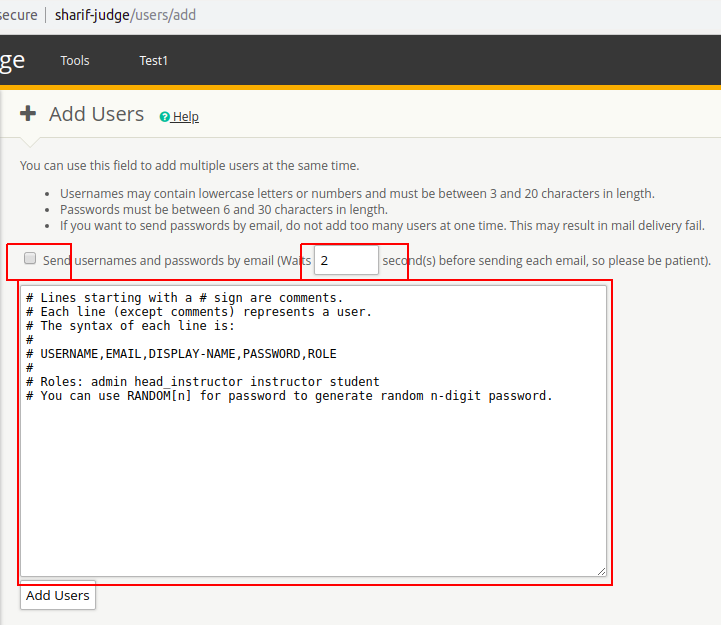
\includegraphics[width=0.5\textwidth]{kepatuhan_1_3_1_add_user}  
				\caption[Kriteria Sukses 1.3.1 - Elemen yang Tidak Diberi Label Pada Halaman \textit{Add Users}]{Kriteria Sukses 1.3.1 - Elemen yang Tidak Diberi Label Pada Halaman \textit{Add Users}} 
				\label{fig:kepatuhan_1_3_1_add_user} 
			\end{figure}
			\item Dalam halaman \textit{Add Assignment} ada elemen dalam form \textit{problems} tidak diberi label. Kesalahan dapat dilihat pada potongan kode \ref{ls_kepatuhan_1_3_1_add_assignment}.
			\begin{lstlisting}[basicstyle=\ttfamily, frame=single,
			columns=fullflexible, keepspaces=true, breaklines=true, label=ls_kepatuhan_1_3_1_add_assignment, caption=Kriteria Sukses 1.3.1 - Elemen Dalam Form yang Tidak Diberi Label]
			...
			<td><input type="text" name="name[]" class="sharif_input short" value="Problem "/></td>\
			...
			\end{lstlisting}
			
			\item Dalam halaman \textit{Problem} terdapat elemen form yang tidak diberi label.
			\begin{figure}[H]
				\centering  
				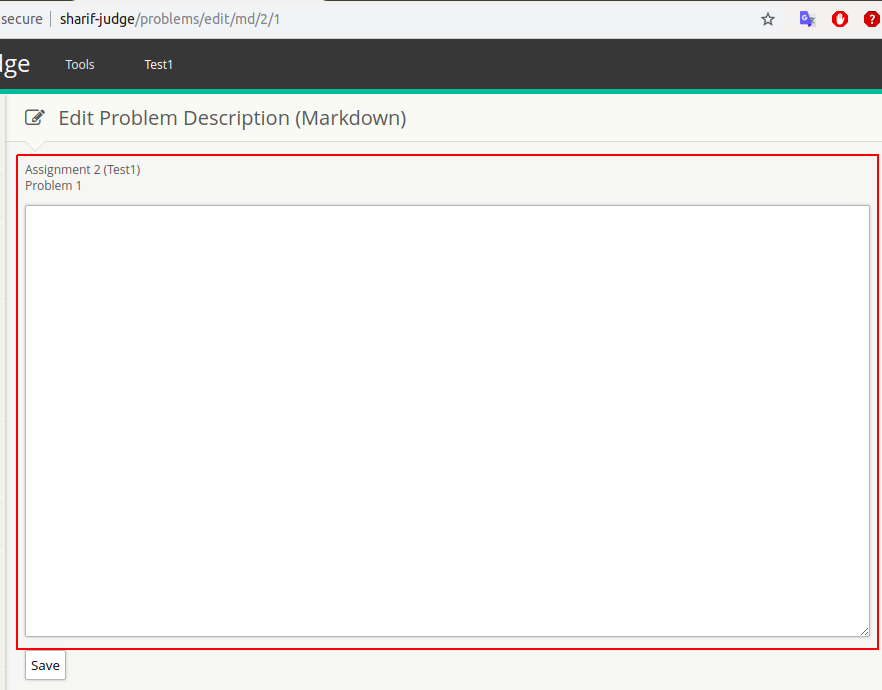
\includegraphics[width=0.5\textwidth]{kepatuhan_1_3_1_problem_edit_markdown}  
				\caption[Kriteria Sukses 1.3.1 - Elemen yang Tidak Diberi Label Pada Halaman \textit{Problems} Bagian \textit{Edit Markdown}]{Kriteria Sukses 1.3.1 - Elemen yang Tidak Diberi Label Pada Halaman \textit{Problems} Bagian \textit{Edit Markdown}} 
				\label{fig:kepatuhan_1_3_1_problem_edit_markdown} 
			\end{figure}
			\begin{figure}[H]
				\centering  
				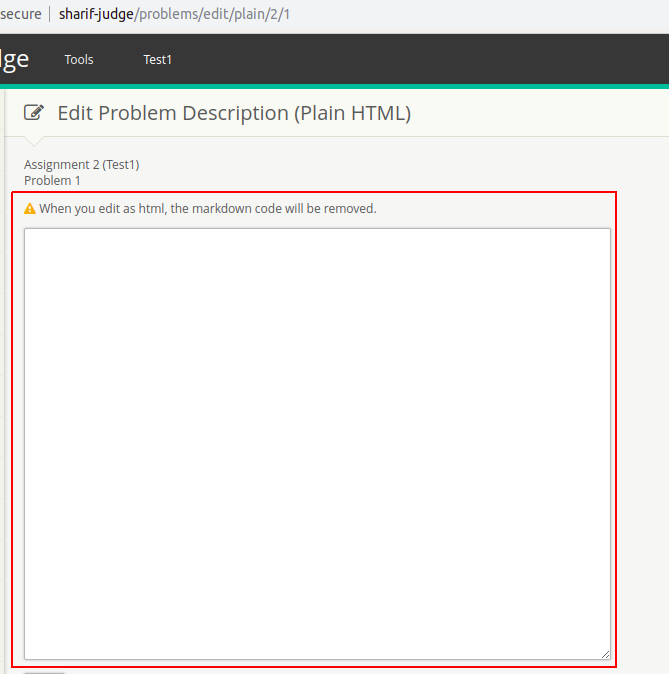
\includegraphics[width=0.5\textwidth]{kepatuhan_1_3_1_edit_plain_html}  
				\caption[Kriteria Sukses 1.3.1 - Elemen yang Tidak Diberi Label Pada Halaman \textit{Problems} Bagian \textit{Edit Plain Html}]{Kriteria Sukses 1.3.1 - Elemen yang Tidak Diberi Label Pada Halaman \textit{Problems} Bagian \textit{Edit Plain Html}} 
				\label{fig:kepatuhan_1_3_1_plain_html} 
			\end{figure}
		\end{itemize}
		
		\subsubsection*{Kriteria Sukses 1.3.2 Meaningful Sequence}
		\label{subsubsec:kepatuhan_kriteria_1.3.2}
		(Sukses) \\
		
		Kriteria ini sukses dipatuhi karena setiap halaman pada \textit{SharIF Judge} memiliki urutan baca dan navigasi yang benar.
		
		\subsubsection*{Kriteria Sukses 1.3.3 Sensory Characteristics}
		\label{subsubsec:kepatuhan_kriteria_1.3.3}
		(Sukses)\\
		
		Kriteria ini sukses dipatuhi karena petunjuk yang diberikan pada aplikasi \textit{SharIF Judge} tidak hanya bergantung pada komponen karakteristik sensorik seperti bentuk, warna, ukuran, lokasi visual, orientasi, atau suara.
		
		\subsubsection*{Kriteria Sukses 1.3.4 Orientation}
		\label{subsubsec:kepatuhan_kriteria_1.3.4}
		(Sukses) \\
		
		Kriteria ini sukses dipatuhi karena konten dari \textit{SharIF Judge} dapat ditampilkan dalam orientasi \textit{portrait} atau \textit{landscape}.
		
		\subsubsection*{Kriteria Sukses 1.3.5 Identify Input Purpose}
		\label{subsubsec:kepatuhan_kriteria_1.3.5}
		(Tidak Sukses)\\
		
		Kriteria ini tidak sukses karena masih ada bidang masukan yang tidak memiliki label, salah satunya pada halaman \textit{Problems} bagian \textit{Edit Markdown}. Kesalahan dapat dilihat pada potongan kode \ref{ls_kepatuhan_1_3_5}.
		\begin{lstlisting}[basicstyle=\ttfamily, frame=single,
		columns=fullflexible, keepspaces=true, breaklines=true, label=ls_kepatuhan_1_3_5, caption=Kriteria Sukses 1.3.5 - Elemen Tidak Diberi Label Pada Halaman \textit{Problems} Bagian \textit{Edit Markdown}]
		...
		<p class="input_p">
		<textarea name="text">{{ problem.description }}</textarea>
		</p>
		...
		\end{lstlisting}
		
		\subsubsection*{Kriteria Sukses 1.3.6 Identify Purpose}
		\label{subsubsec:kepatuhan_kriteria_1.3.6}
		(Tidak Sukses) \\
		
		Kriteria ini tidak sukses dipatuhi karena ada elemen \textit{HTML} yang seharusnya dapat dipakai tetapi tidak digunakan, seperti bagian navigasi dan judul bagian. Kesalahan dapat dilihat pada potongan kode \ref{ls_kepatuhan_1_3_6}.
		\begin{lstlisting}[basicstyle=\ttfamily, frame=single,
		columns=fullflexible, keepspaces=true, breaklines=true, label=ls_kepatuhan_1_3_6, caption=Kriteria Sukses 1.3.6 - \textit{Sidebar}]
		...
		<div id="side_bar" class="sidebar_open">
		<ul>
		<li class="color-dashboard{{ selected=='dashboard' ? ' selected' }}">
		...
		\end{lstlisting}
		
		\subsubsection*{Kriteria Sukses 1.4.1 Use of Color}
		\label{subsubsec:kepatuhan_kriteria_1.4.1}
		(Sukses) \\
		
		Kriteria ini sukses dipatuhi karena warna tidak digunakan sebagai satu-satunya cara untuk menyampaikan informasi, menunjukkan aksi, menampilkan respon, atau membedakan elemen visual. Selain warna, ada juga teks yang menjelaskan informasi yang ditampilkan.
		
		\subsubsection*{Kriteria Sukses 1.4.2 Audio Control}
		\label{subsubsec:kepatuhan_kriteria_1.4.2}
		(Sukses) \\
		
		Kriteria ini sukses dipatuhi karena pada aplikasi \textit{SharIF Judge} tidak terdapat konten berbasis waktu.
		
		\subsubsection*{Kriteria Sukses 1.4.3 Contrast (Minimum)}
		\label{subsubsec:kepatuhan_kriteria_1.4.3}
		(Tidak Sukses) \\
		
		Kriteria ini tidak sukses dipatuhi karena pada aplikasi \textit{SharIF Judge} terdapat beberapa teks dengan rasio kontras kurang dari 4.5:1, antara lain:
		\begin{itemize}
			\item Navigasi Atas: Teks tempat waktu yang tersisa untuk mengumpulkan suatu \textit{Assignment} memiliki rasio kontras 2.52:1 terhadap warna latar belakangnya. Tampilan halaman web dapat dilihat pada gambar \ref{fig:kepatuhan_1_4_3_navigasi_atas}.
			\begin{figure}[H]
				\centering  
				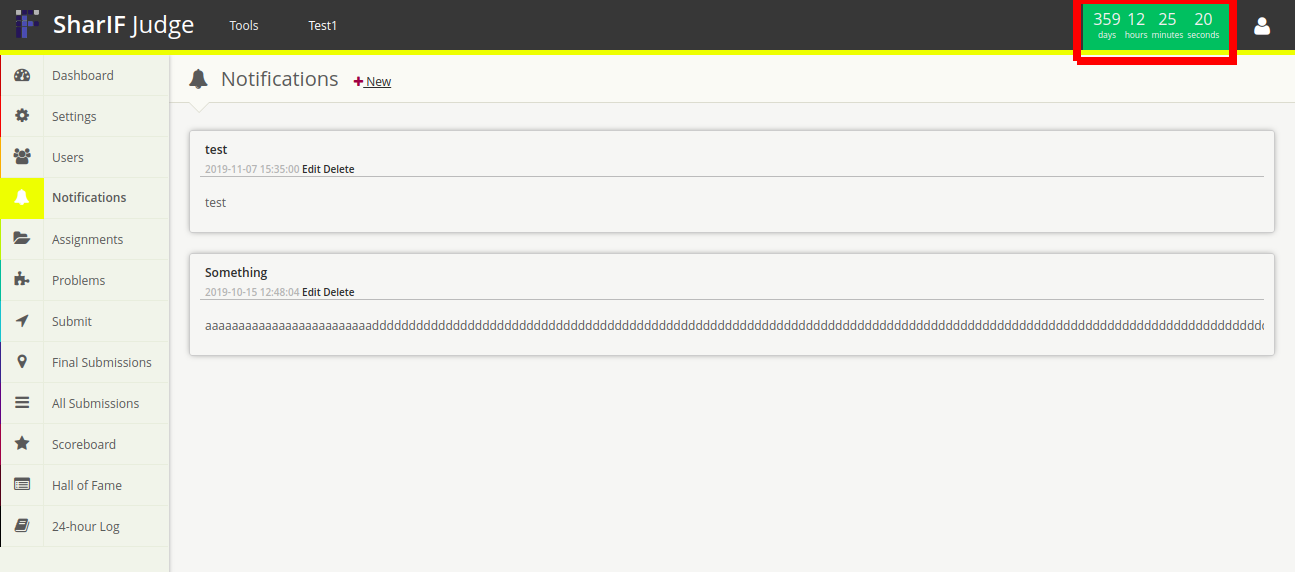
\includegraphics[scale=0.25]{kepatuhan_1_4_3_navigasi_atas}  
				\caption[Kriteria Sukses 1.4.3 - Kontras Elemen Navigasi Atas]{Kriteria Sukses 1.4.3 - Kontras Elemen Navigasi Atas} 
				\label{fig:kepatuhan_1_4_3_navigasi_atas} 
			\end{figure}
			
			\item Halaman \textit{Dashboard}: Teks pada tombol \textit{today} memiliki rasio kontras 4.01:1 terhadap warna latar belakangnya. Teks pada kalender memiliki rasio kontras 2.69:1 terhadap warna latar belakangnya. Teks pada kalender yang menunjukkan tanggal memiliki rasio kontras 1.57:1 terhadap warna latar belakangnya. Teks yang menunjukkan waktu notifikasi dibuat memiliki rasio kontras 2.07:1 terhadap warna latar belakangnya. Tampilan halaman web dapat dilihat pada gambar \ref{fig:kepatuhan_1_4_3_dashboard}.
			\begin{figure}[H]
				\centering  
				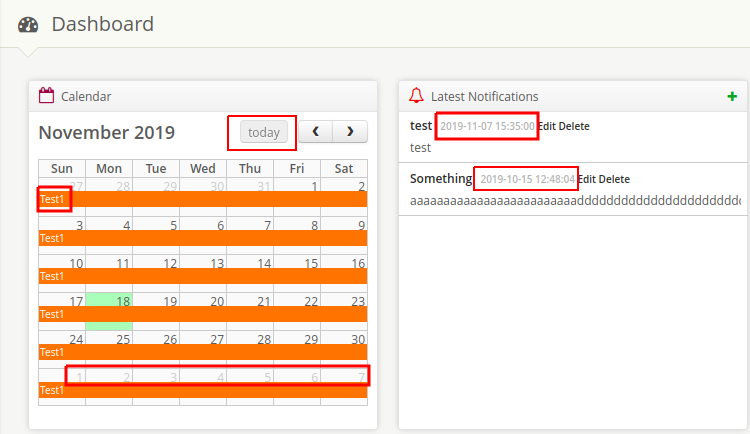
\includegraphics[scale=0.5]{kepatuhan_1_4_3_dashboard}  
				\caption[Kriteria Sukses 1.4.3 - Kontras Elemen Dashboard]{Kriteria Sukses 1.4.3 - Kontras Elemen Dashboard} 
				\label{fig:kepatuhan_1_4_3_dashboard} 
			\end{figure}
			
			\item Halaman \textit{Settings}: Informasi tambahan pada bidang masukkan memiliki rasio kontras 3.55:1 terhadap warna latar belakangnya. Informasi peringatan pada bidang masukkan memiliki rasio kontras 3.69:1 terhadap warna latar belakangnya. Tampilan halaman web dapat dilihat pada gambar \ref{fig:kepatuhan_1_4_3_settings}.
			\begin{figure}[H]
				\centering  
				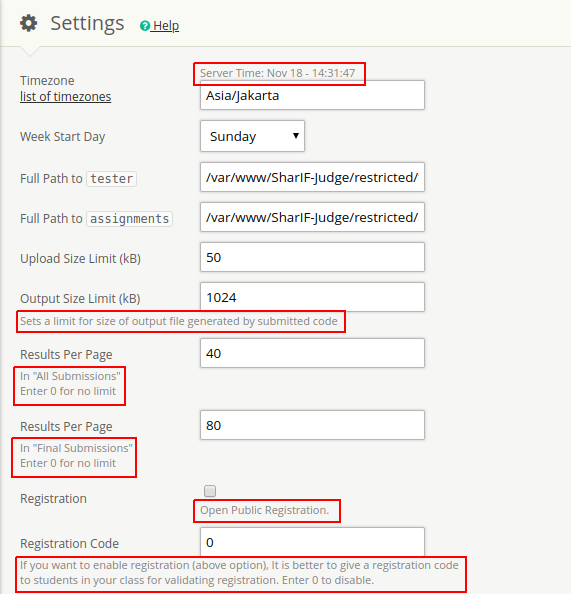
\includegraphics[scale=0.5]{kepatuhan_1_4_3_settings}  
				\caption[Kriteria Sukses 1.4.3 - Kontras Elemen Settings]{Kriteria Sukses 1.4.3 - Kontras Elemen Settings} 
				\label{fig:kepatuhan_1_4_3_settings} 
			\end{figure}
			
			\item Halaman \textit{Notifications}: Teks yang menunjukkan waktu notifikasi dibuat memiliki rasio kontras 1.91:1 terhadap warna latar belakangnya. Tampilan halaman web dapat dilihat pada gambar \ref{fig:kepatuhan_1_4_3_notifications}.
			\begin{figure}[H]
				\centering  
				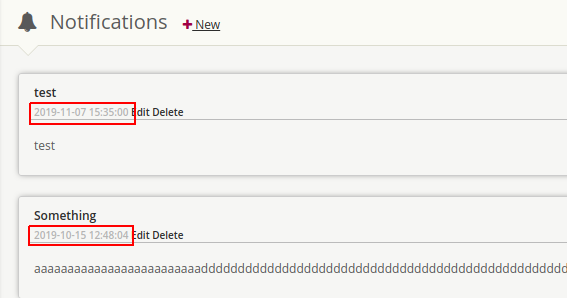
\includegraphics[scale=0.5]{kepatuhan_1_4_3_notifications}  
				\caption[Kriteria Sukses 1.4.3 - Kontras Elemen Notifications]{Kriteria Sukses 1.4.3 - Kontras Elemen Notifications} 
				\label{fig:kepatuhan_1_4_3_notifications} 
			\end{figure}
			
			\item Halaman \textit{Assignment}: Teks yang berwana merah pada tabel \textit{Assignment} memiliki rasio kontras 3.89:1 terhadap warna latar belakangnya. Tampilan halaman web dapat dilihat pada gambar \ref{fig:kepatuhan_1_4_3_assignments}.
			\begin{figure}[H]
				\centering  
				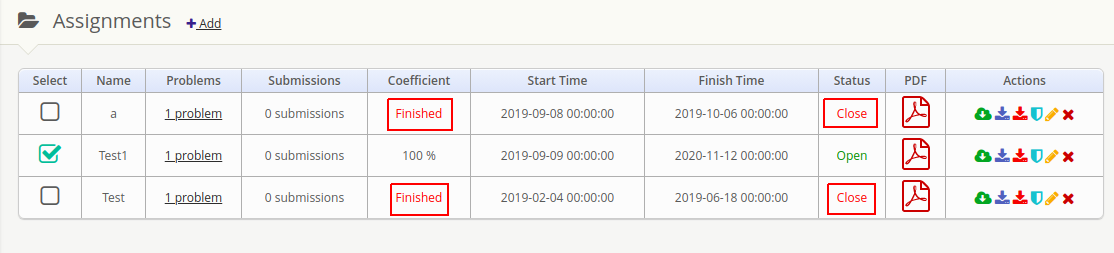
\includegraphics[scale=0.3]{kepatuhan_1_4_3_assignments}  
				\caption[Kriteria Sukses 1.4.3 - Kontras Elemen Assignments]{Kriteria Sukses 1.4.3 - Kontras Elemen Assignments} 
				\label{fig:kepatuhan_1_4_3_assignments} 
			\end{figure}
			
			\item Halaman \textit{Add Assignment}: Informasi tambahan pada bidang masukkan memiliki rasio kontras 3.55:1 terhadap warna latar belakangnya. Informasi peringatan pada bidang masukkan memiliki rasio kontras 3.69:1 terhadap warna latar belakangnya. Tampilan halaman web dapat dilihat pada gambar \ref{fig:kepatuhan_1_4_3_add_assignment}.
			\begin{figure}[H]
				\centering  
				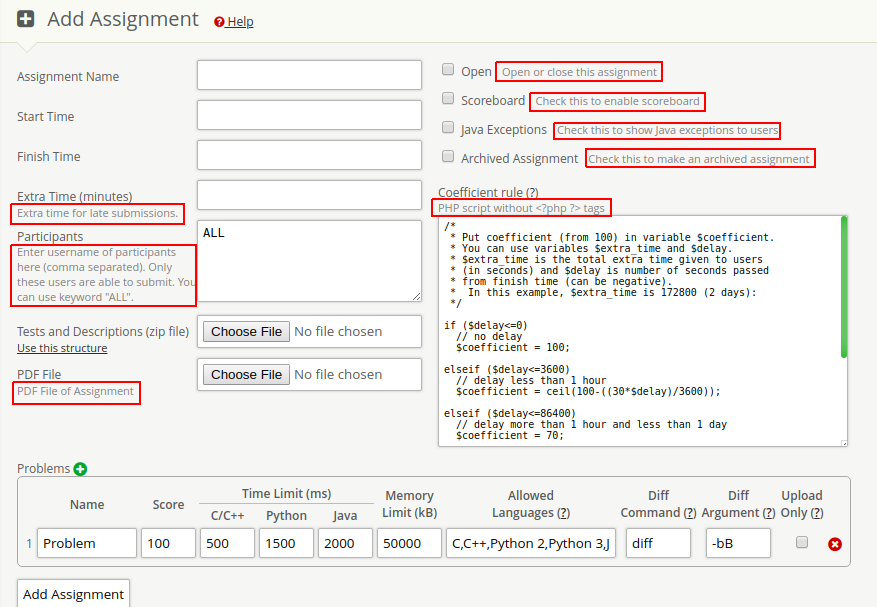
\includegraphics[scale=0.5]{kepatuhan_1_4_3_add_assignment}  
				\caption[Kriteria Sukses 1.4.3 - Kontras Elemen \textit{Add Assignments}]{Kriteria Sukses 1.4.3 - Kontras Elemen \textit{Add Assignments}} 
				\label{fig:kepatuhan_1_4_3_add_assignment} 
			\end{figure}
			
		\end{itemize}
		
		\subsubsection*{Kriteria Sukses 1.4.4 Resize text}
		\label{subsubsec:kepatuhan_kriteria_1.4.4}
		(Tidak Sukses) \\
		
		Kriteria ini tidak sukses dipatuhi karena fungsionalitas \textit{navigation bar} tidak berjalan pada pembesaran 125 persen. Tampilan halaman web dapat dilihat pada gambar \ref{fig:kepatuhan_1_4_4_nav_bar}.
		\begin{figure}[H]
			\centering  
			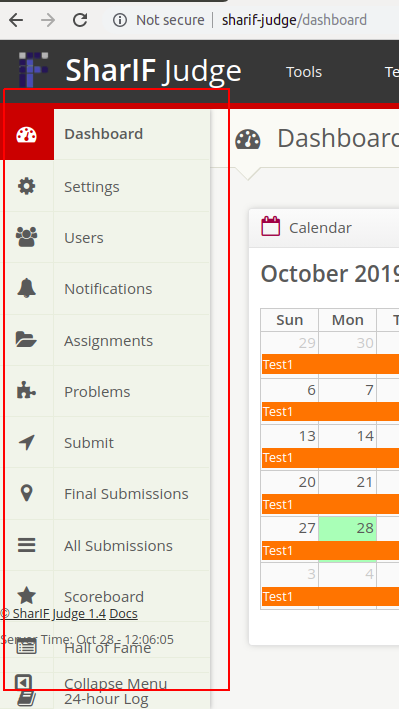
\includegraphics[width=0.5\textwidth]{kepatuhan_1_4_4_nav_bar}  
			\caption[Kriteria Sukses 1.4.4 - Sidenav]{Kriteria Sukses 1.4.4 - Sidenav} 
			\label{fig:kepatuhan_1_4_4_nav_bar} 
		\end{figure}
		
		
		\subsubsection*{Kriteria Sukses 1.4.5 Images of Text}
		\label{subsubsec:kepatuhan_kriteria_1.4.5}
		(Sukses) \\
		
		Kriteria ini sukses dipatuhi karena semua gambar teks yang ada pada aplikasi \textit{SharIF Judge} penting untuk informasi yang disampaikan.
		
		\subsubsection*{Kriteria Sukses 1.4.6 Contrast (Enhanced)}
		\label{subsubsec:kepatuhan_kriteria_1.4.6}
		
		(Tidak Sukses) \\
		
		Kriteria ini tidak sukses dipatuhi karena pada aplikasi \textit{SharIF Judge} terdapat beberapa teks dengan rasio kontras kurang dari 4.5:1, antara lain:
		\begin{itemize}
			\item Navigasi Atas: Teks tempat waktu yang tersisa untuk mengumpulkan suatu \textit{Assignment} memiliki rasio kontras 2.52:1 terhadap warna latar belakangnya. Tampilan halaman web dapat dilihat pada gambar \ref{fig:kepatuhan_1_4_6_navigasi_atas}.
			\begin{figure}[H]
				\centering  
				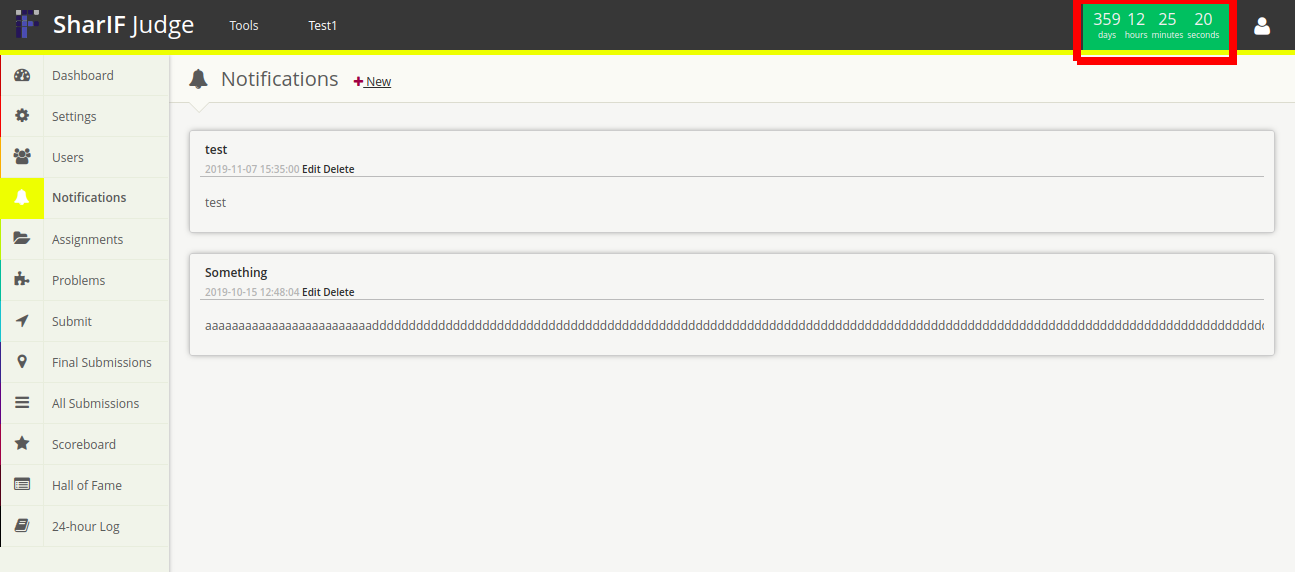
\includegraphics[scale=0.25]{kepatuhan_1_4_6_navigasi_atas}  
				\caption[Kriteria Sukses 1.4.6 - Kontras Elemen Navigasi Atas]{Kriteria Sukses 1.4.6 - Kontras Elemen Navigasi Atas} 
				\label{fig:kepatuhan_1_4_6_navigasi_atas} 
			\end{figure}
			
			\item Halaman \textit{Dashboard}: Teks pada tombol \textit{today} memiliki rasio kontras 4.01:1 terhadap warna latar belakangnya. Teks pada kalender memiliki rasio kontras 2.69:1 terhadap warna latar belakangnya. Teks pada kalender yang menunjukkan tanggal memiliki rasio kontras 1.57:1 terhadap warna latar belakangnya. Teks yang menunjukkan waktu notifikasi dibuat memiliki rasio kontras 2.07:1 terhadap warna latar belakangnya. Tampilan halaman web dapat dilihat pada gambar \ref{fig:kepatuhan_1_4_6_dashboard}.
			\begin{figure}[H]
				\centering  
				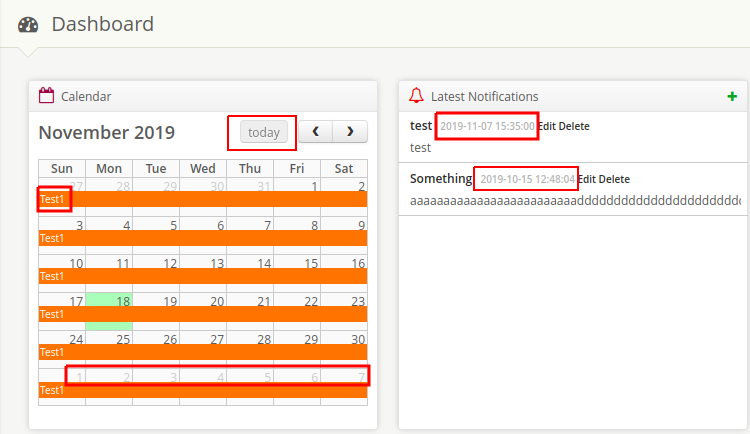
\includegraphics[scale=0.5]{kepatuhan_1_4_6_dashboard}  
				\caption[Kriteria Sukses 1.4.6 - Kontras Elemen Dashboard]{Kriteria Sukses 1.4.6 - Kontras Elemen Dashboard} 
				\label{fig:kepatuhan_1_4_6_dashboard} 
			\end{figure}
			
			\item Halaman \textit{Settings}: Informasi tambahan pada bidang masukkan memiliki rasio kontras 3.55:1 terhadap warna latar belakangnya. Informasi peringatan pada bidang masukkan memiliki rasio kontras 3.69:1 terhadap warna latar belakangnya. Tampilan halaman web dapat dilihat pada gambar \ref{fig:kepatuhan_1_4_6_settings}.
			\begin{figure}[H]
				\centering  
				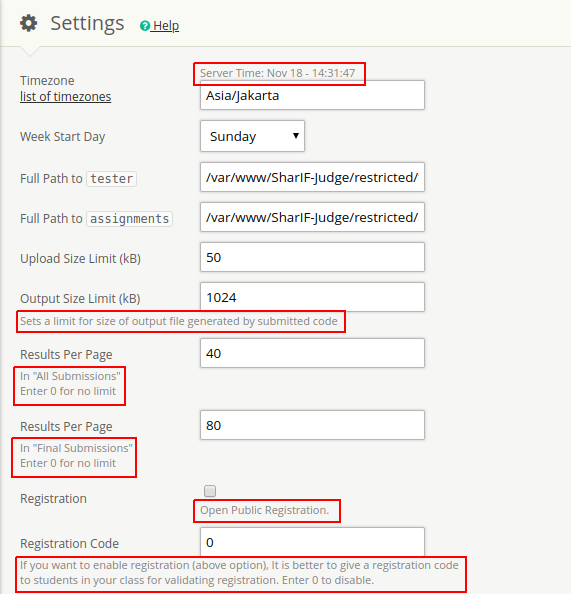
\includegraphics[scale=0.5]{kepatuhan_1_4_6_settings}  
				\caption[Kriteria Sukses 1.4.6 - Kontras Elemen Settings]{Kriteria Sukses 1.4.6 - Kontras Elemen Settings} 
				\label{fig:kepatuhan_1_4_6_settings} 
			\end{figure}
			
			\item Halaman \textit{Notifications}: Teks yang menunjukkan waktu notifikasi dibuat memiliki rasio kontras 1.91:1 terhadap warna latar belakangnya. Tampilan halaman web dapat dilihat pada gambar \ref{fig:kepatuhan_1_4_6_notifications}.
			\begin{figure}[H]
				\centering  
				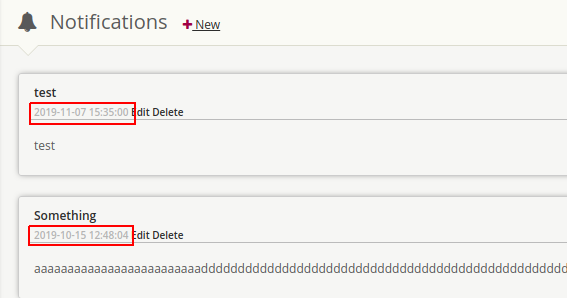
\includegraphics[scale=0.5]{kepatuhan_1_4_6_notifications}  
				\caption[Kriteria Sukses 1.4.6 - Kontras Elemen Notifications]{Kriteria Sukses 1.4.6 - Kontras Elemen Notifications} 
				\label{fig:kepatuhan_1_4_6_notifications} 
			\end{figure}
			
			\item Halaman \textit{Assignment}: Teks yang berwana merah pada tabel \textit{Assignment} memiliki rasio kontras 3.89:1 terhadap warna latar belakangnya. Tampilan halaman web dapat dilihat pada gambar \ref{fig:kepatuhan_1_4_6_assignments}.
			\begin{figure}[H]
				\centering  
				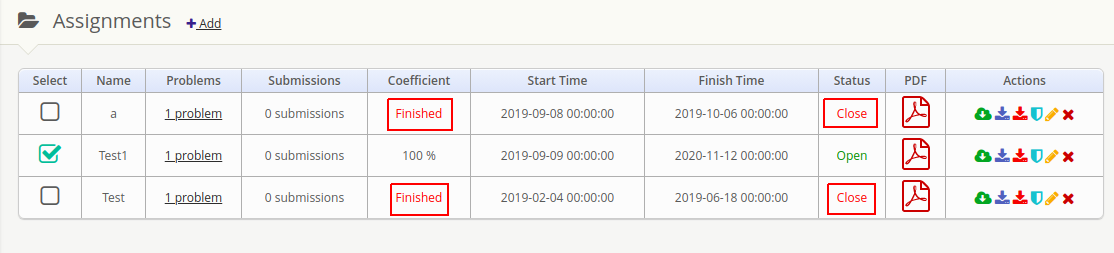
\includegraphics[scale=0.3]{kepatuhan_1_4_6_assignments}  
				\caption[Kriteria Sukses 1.4.6 - Kontras Elemen Assignments]{Kriteria Sukses 1.4.6 - Kontras Elemen Assignments} 
				\label{fig:kepatuhan_1_4_6_assignments} 
			\end{figure}
			
			\item Halaman \textit{Add Assignment}: Informasi tambahan pada bidang masukkan memiliki rasio kontras 3.55:1 terhadap warna latar belakangnya. Informasi peringatan pada bidang masukkan memiliki rasio kontras 3.69:1 terhadap warna latar belakangnya. Tampilan halaman web dapat dilihat pada gambar \ref{fig:kepatuhan_1_4_6_add_assignment}.
			\begin{figure}[H]
				\centering  
				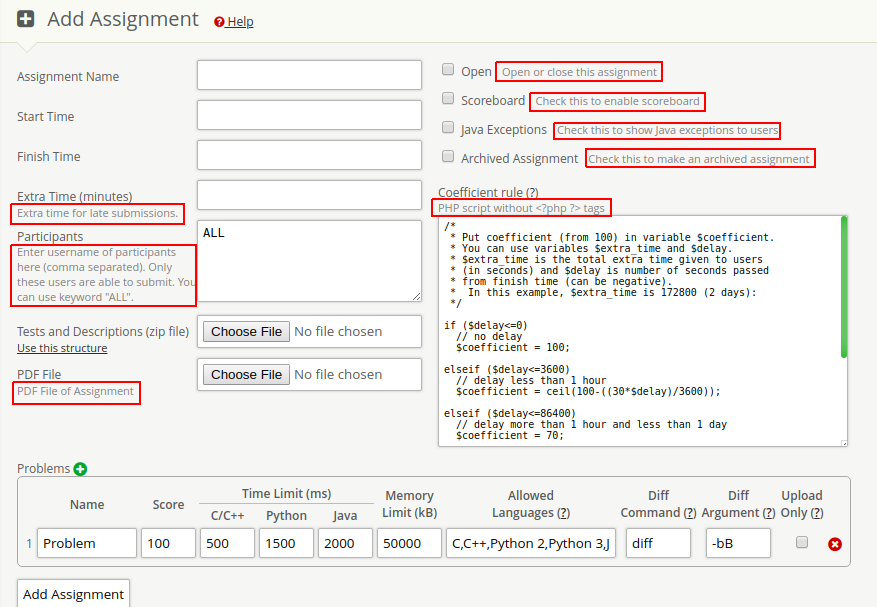
\includegraphics[scale=0.5]{kepatuhan_1_4_6_add_assignment}  
				\caption[Kriteria Sukses 1.4.6 - Kontras Elemen Add Assignments]{Kriteria Sukses 1.4.6 - Kontras Elemen Add Assignments} 
				\label{fig:kepatuhan_1_4_6_add_assignment} 
			\end{figure}
			
		\end{itemize}
		
		\subsubsection*{Kriteria Sukses 1.4.7 Low atau No Background Audio}
		\label{subsubsec:kepatuhan_kriteria_1.4.7}
		(Sukses) \\
		
		Kriteria ini sukses dipatuhi karena pada aplikasi \textit{SharIF Judge} tidak terdapat konten berbasis waktu.
		
		
		\subsubsection*{Kriteria Sukses 1.4.8 Visual Presentation}
		\label{subsubsec:kepatuhan_kriteria_1.4.8}
		(Tidak Sukses) \\
		
		Kriteria ini tidak sukses dipatuhi karena pada halaman \textit{Dashboard} dan \textit{Notifications} teks yang menampilkan isi notifikasi memiliki lebar lebih dari 80 karakter. Tampilan halaman web ditampilkan pada gambar \ref{fig:kepatuhan_1_4_8_notifications}.
		\begin{figure}[H]
			\centering  
			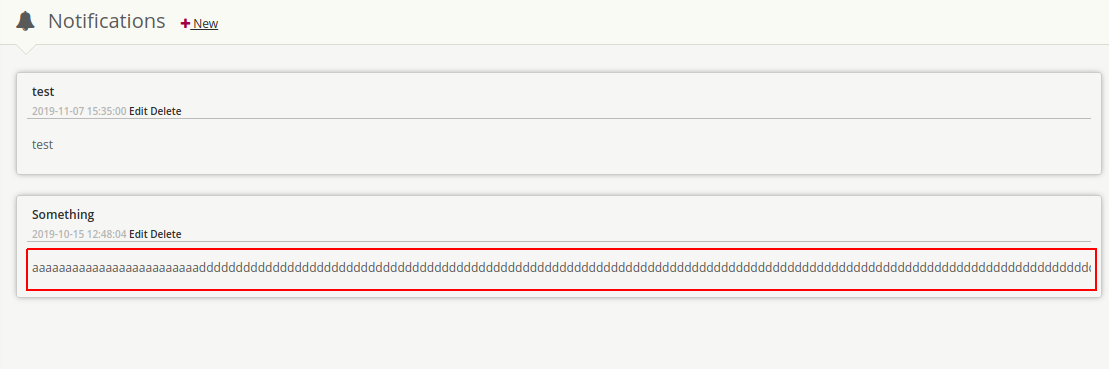
\includegraphics[scale=0.25]{kepatuhan_1_4_8_notifications}  
			\caption[Kriteria Sukses 1.4.8 - Notifications]{Kriteria Sukses 1.4.8 - Notifications} 
			\label{fig:kepatuhan_1_4_8_notifications} 
		\end{figure}
		
		\subsubsection*{Kriteria Sukses 1.4.9 Images of Text (No Exception)}
		\label{subsubsec:kepatuhan_kriteria_1.4.9}
		(Sukses) \\
		
		Kriteria ini sukses dipatuhi karena semua gambar teks yang ada pada aplikasi \textit{SharIF Judge} penting untuk informasi yang disampaikan.
		
		\subsubsection*{Kriteria Sukses 1.4.10 Reflow}
		\label{subsubsec:kepatuhan_kriteria_1.4.10}
		(Tidak Sukses) \\
		
		Kriteria ini tidak sukses dipatuhi karena pada setiap halaman aplikasi \textit{SharIF Judge} memerlukan \textit{scroll} secara horizontal ketika ditampilkan pada resolusi layar 1280 pixel dengan pembesaran 400 persen. Tampilan halaman web dapat dilihat pada gambar \ref{fig:kepatuhan_1_4_10_reflow}
		\begin{figure}[H]
			\centering  
			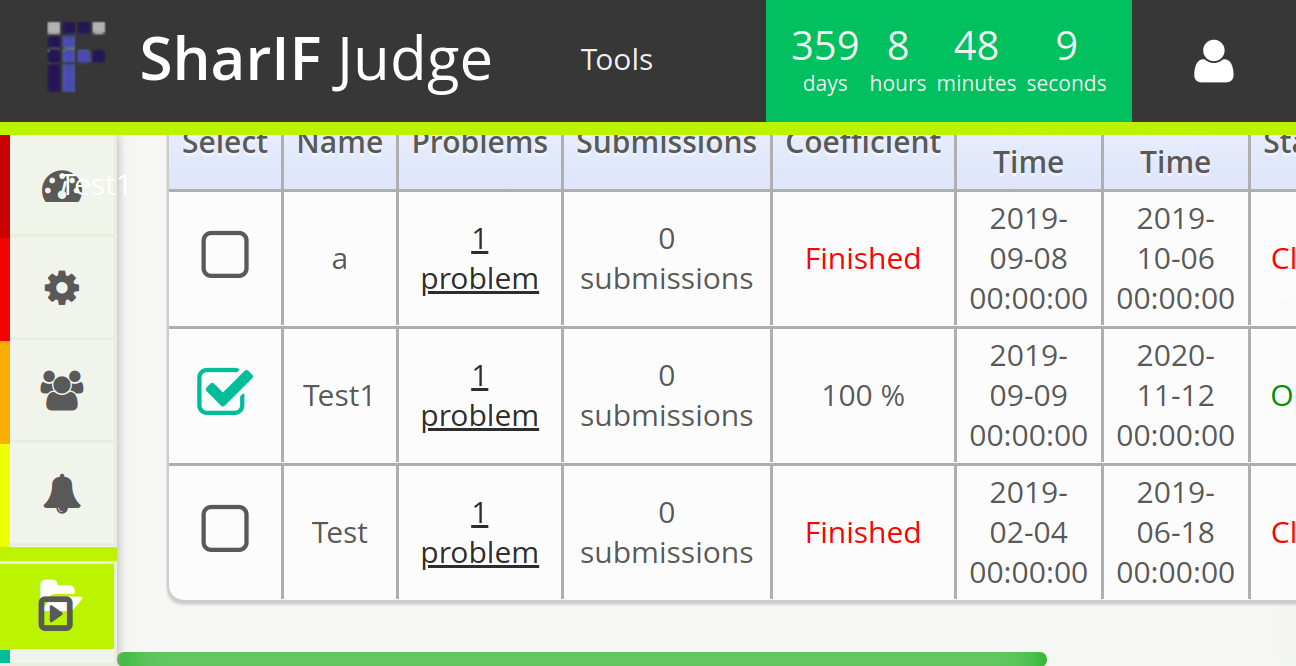
\includegraphics[scale=0.25]{kepatuhan_1_4_10}  
			\caption[Kriteria Sukses 1.4.10 - Horizontal \textit{Scroll}]{Kriteria Sukses 1.4.10 - Horizontal \textit{Scroll}} 
			\label{fig:kepatuhan_1_4_10_reflow} 
		\end{figure}
		
		\subsubsection*{Kriteria Sukses 1.4.11 Non-text Contrast}
		\label{subsubsec:kepatuhan_kriteria_1.4.11}
		(Diabaikan) \\
		
		Kriteria ini diabaikan karena pengukuran kontras sulit untuk dilakukan. Tampilan halaman web dapat dilihat pada gambar \ref{fig:kepatuhan_1_4_11_reflow}.
		\begin{figure}[H]
			\centering  
			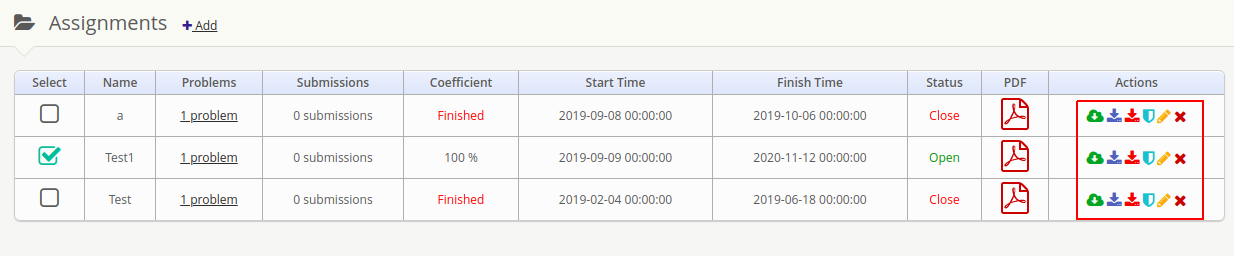
\includegraphics[scale=0.3]{kepatuhan_1_4_11}  
			\caption[Kriteria Sukses 1.4.11 - Ikon Pada Halaman \textit{Assignments}]{Kriteria Sukses 1.4.11 - Ikon Pada Halaman \textit{Assignments}} 
			\label{fig:kepatuhan_1_4_11_reflow} 
		\end{figure}
		
		\subsubsection*{Kriteria Sukses 1.4.12 Text Spacing}
		\label{subsubsec:kepatuhan_kriteria_1.4.12}
		(Sukses) \\
		
		Kriteria ini sukses dipatuhi karena penulis telah melakukan uji coba pada salah satu halaman agar kriteria ini terpenuhi dan hasilnya tidak terjadi masalah. Oleh karena itu, penulis menyimpulkan bahwa jika perubahan dilakukan di halaman lain akan menghasilkan hal yang sama. Tampilan halaman web dapat dilihat pada gambar \ref{fig:kepatuhan_1_4_12}.
		\begin{figure}[H]
			\centering  
			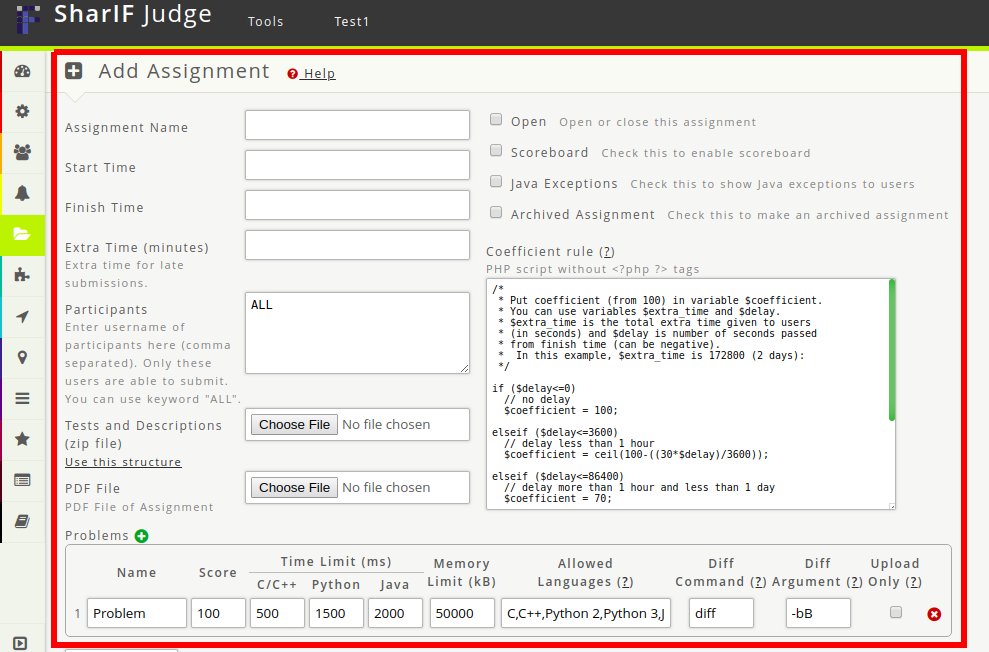
\includegraphics[scale=0.3]{kepatuhan_1_4_12}  
			\caption[Kriteria Sukses 1.4.12 - Halaman \textit{Add Assignment}]{Kriteria Sukses 1.4.12 - Halaman \textit{Add Assignment}} 
			\label{fig:kepatuhan_1_4_12} 
		\end{figure}
	
		\subsubsection*{Kriteria Sukses 1.4.13 Content on Hover or Focus}
		\label{subsubsec:kepatuhan_kriteria_1.4.13}
		(Sukses) \\
		
		Kriteria ini sukses dipatuhi karena setiap konten tambahan yang muncul sesaat ketika suatu elemen menerima penunjuk kursor atau fokus \textit{keyboard}, konten tambahan tersebut dapat disingkirkan, dapat ditunjuk, dan persisten.
		
		\subsection*{\textit{Operable}}
		\label{subsec:kepatuhan_operable}
		
		\subsubsection*{Kriteria Sukses 2.1.1 Keyboard}
		\label{subsubsec:kepatuhan_kriteria_2.1.1}
		(Tidak Sukses) \\
		
		Kriteria ini tidak sukses dipatuhi karena :
		\begin{itemize}
			\item Tombol \textit{Collapse Menu} pada \textit{sidebar} tidak dapat dioperasikan dengan keyboard. Tampilan halaman web dapat dilihat pada gambar \ref{fig:kepatuhan_2_1_1_collapse_menu}.
			\begin{figure}[H]
				\centering  
				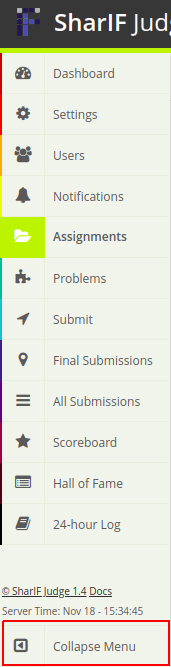
\includegraphics[scale=0.5]{kepatuhan_2_1_1_collapse_menu}  
				\caption[Kriteria Sukses 2.1.1 - \textit{Collapse Menu}]{Kriteria Sukses 2.1.1 - \textit{Collapse Menu}} 
				\label{fig:kepatuhan_2_1_1_collapse_menu} 
			\end{figure}
			
			\item Tombol \textit{Tools} pada \textit{Menu} tidak dapat dioperasikan dengan keyboard. Tampilan halaman web dapat dilihat pada gambar \ref{fig:kepatuhan_2_1_1_tools}.
			\begin{figure}[H]
				\centering  
				
\includegraphics[scale=0.5]{kepatuhan_2_1_1_tools}  
				\caption[Kriteria Sukses 2.1.1 - \textit{Tools}]{Kriteria Sukses 2.1.1 - \textit{Tools}} 
				\label{fig:kepatuhan_2_1_1_tools} 
			\end{figure}
			
		\end{itemize}
		
		\subsubsection*{Kriteria Sukses 2.1.2 No Keyboard Trap}
		\label{subsubsec:kepatuhan_kriteria_2.1.2}
		(Tidak Sukses) \\
		
		Kriteria ini tidak sukses dipatuhi karena :
		\begin{itemize}
			\item Dalam halaman \textit{Settings} ada \textit{input field} yang fokusnya tidak dapat dipindahkan menggunakan antarmuka \textit{keyboard}. \textit{Input field} yang dimaksud dapat dilihat pada gambar \ref{fig:kepatuhan_2_1_2_settings}.
			\begin{figure}[H]
				\centering  
				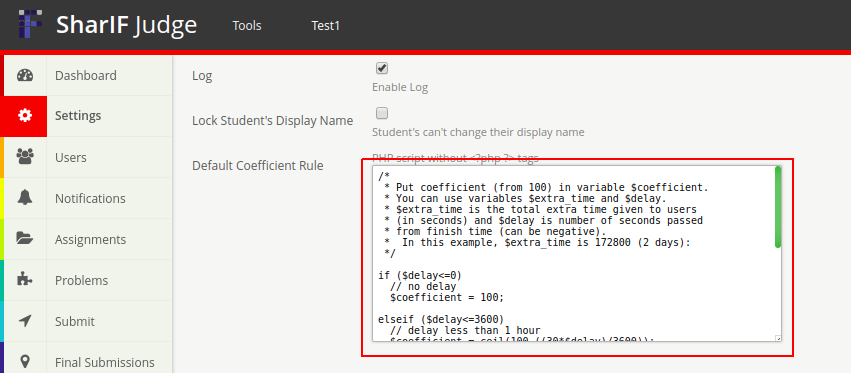
\includegraphics[scale=0.5]{kepatuhan_2_1_2_settings}  
				\caption[Kriteria Sukses 2.1.2 - \textit{Settings}]{Kriteria Sukses 2.1.2 - \textit{Settings}} 
				\label{fig:kepatuhan_2_1_2_settings} 
			\end{figure}
			
			\item Dalam halaman \textit{Add User} ada \textit{input field} yang fokusnya tidak dapat dipindahkan menggunakan antarmuka \textit{keyboard}.\textit{Input field} yang dimaksud dapat dilihat pada gambar \ref{fig:kepatuhan_2_1_2_add_user}.
			\begin{figure}[H]
				\centering  
				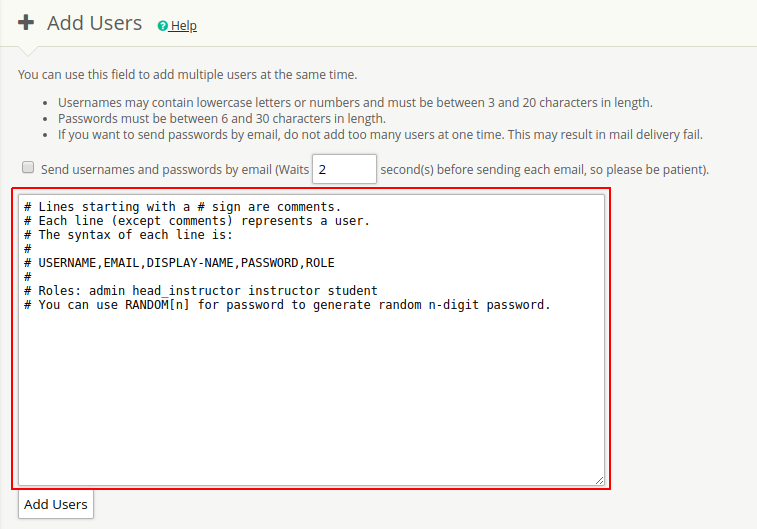
\includegraphics[scale=0.5]{kepatuhan_2_1_2_add_user}  
				\caption[Kriteria Sukses 2.1.2 - \textit{Add User}]{Kriteria Sukses 2.1.2 - \textit{Add User}} 
				\label{fig:kepatuhan_2_1_2_add_user} 
			\end{figure}
			
			\item Dalam halaman \textit{Add Assignment} ada \textit{input field} yang fokusnya tidak dapat dipindahkan menggunakan antarmuka \textit{keyboard}.\textit{Input field} yang dimaksud dapat dilihat pada gambar \ref{fig:kepatuhan_2_1_2_add_assignment}.
			\begin{figure}[H]
				\centering  
				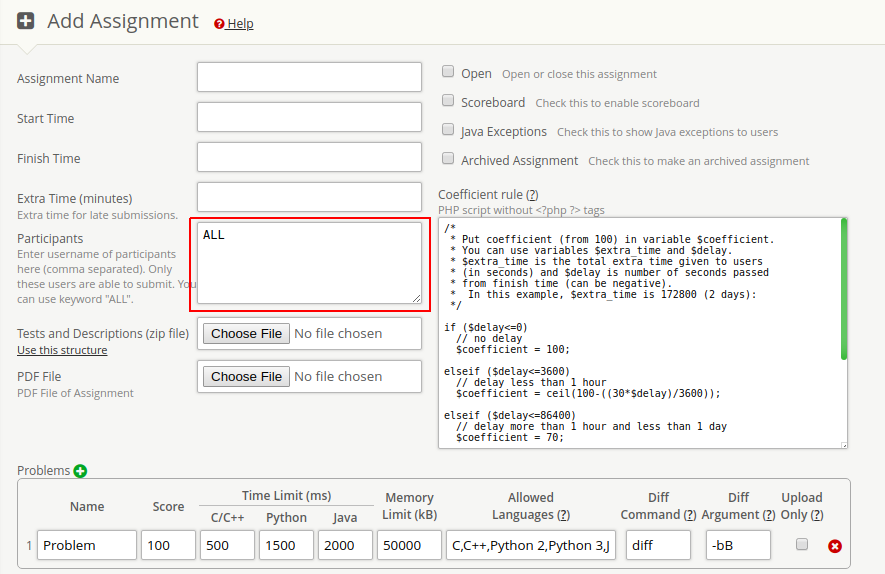
\includegraphics[scale=0.5]{kepatuhan_2_1_2_add_assignment}  
				\caption[Kriteria Sukses 2.1.2 - \textit{Add Assignment}]{Kriteria Sukses 2.1.2 - \textit{Add Assignment}} 
				\label{fig:kepatuhan_2_1_2_add_assignment} 
			\end{figure}
			
			\item Dalam halaman \textit{Problems}(\textit{Edit Markdown}) ada \textit{input field} yang fokusnya tidak dapat dipindahkan menggunakan antarmuka \textit{keyboard}.\textit{Input field} yang dimaksud dapat dilihat pada gambar \ref{fig:kepatuhan_2_1_2_problems_edit_markdown}.
			\begin{figure}[H]
				\centering  
				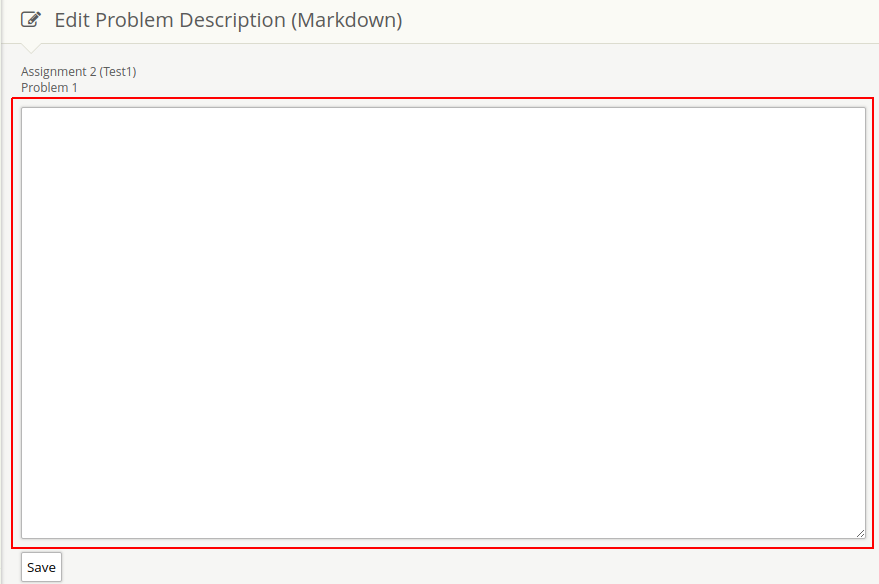
\includegraphics[scale=0.5]{kepatuhan_2_1_2_problems_edit_markdown}  
				\caption[Kriteria Sukses 2.1.2 - \textit{Problems} Bagian \textit{Edit Markdown}]{Kriteria Sukses 2.1.2 - \textit{Problems} Bagian \textit{Edit Markdown}} 
				\label{fig:kepatuhan_2_1_2_problems_edit_markdown} 
			\end{figure}
			
		\end{itemize}
		
		\subsubsection*{Kriteria Sukses 2.1.3 Keyboard (No Exception)}
		\label{subsubsec:kepatuhan_kriteria_2.1.3}
		(Tidak Sukses) \\
		
		Kriteria ini tidak sukses dipatuhi karena :
		\begin{itemize}
			\item Tombol \textit{Collapse Menu} pada \textit{sidebar} tidak dapat dioperasikan dengan keyboard. Tampilan halaman web dapat dilihat pada gambar \ref{fig:kepatuhan_2_1_3_collapse_menu}.
			\begin{figure}[H]
				\centering  
				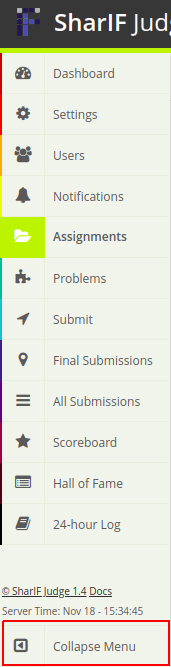
\includegraphics[scale=0.5]{kepatuhan_2_1_3_collapse_menu}  
				\caption[Kriteria Sukses 2.1.3 - \textit{Collapse Menu}]{Kriteria Sukses 2.1.3 - \textit{Collapse Menu}} 
				\label{fig:kepatuhan_2_1_3_collapse_menu} 
			\end{figure}
			
			\item Tombol \textit{Tools} dan \textit{Assignments} pada \textit{Menu} tidak dapat dioperasikan dengan keyboard. Tampilan halaman web dapat dilihat pada gambar \ref{fig:kepatuhan_2_1_3_tools}.
			\begin{figure}[H]
				\centering  
				
\includegraphics[scale=0.5]{kepatuhan_2_1_3_tools}  
				\caption[Kriteria Sukses 2.1.3 - \textit{Tools}]{Kriteria Sukses 2.1.3 - \textit{Tools}} 
				\label{fig:kepatuhan_2_1_3_tools} 
			\end{figure}
			
		\end{itemize}
		
		\subsubsection*{Kriteria Sukses 2.1.4 Character Key Shortcuts}
		\label{subsubsec:kepatuhan_kriteria_2.1.4}
		(Sukses) \\
		
		Kriteria ini sukses dipatuhi karena pada aplikasi \textit{SharIF Judge} tidak terdapat pintasan \textit{keyboard} untuk konten yang ditampilkan.
		
		\subsubsection*{Kriteria Sukses 2.2.1 Timing Adjustable}
		\label{subsubsec:kepatuhan_kriteria_2.2.1}
		(Sukses) \\
		
		Kriteria ini sukses dipatuhi karena pada aplikasi \textit{SharIF Judge} batas waktu untuk mengumpulkan \textit{Assignment} merupakan hal yang esensial dan perpanjangan batas waktu menyalahi inti dari kegiatan tersebut.
		
		\subsubsection*{Kriteria Sukses 2.2.2 Pause, Stop, Hide}
		\label{subsubsec:kepatuhan_kriteria_2.2.2}
		(Sukses) \\
		
		Kriteria ini sukses dipatuhi karena pada aplikasi \textit{SharIF Judge} satu-satunya informasi yang diperbarui secara otomatis adalah batas waktu pengumpulan \textit{Assignment} yang merupakan bagian dari aktivitas yang esensial.
		
		\subsubsection*{Kriteria Sukses 2.2.3 No Timing}
		\label{subsubsec:kepatuhan_kriteria_2.2.3}
		(Sukses) \\
		
		Kriteria ini sukses dipatuhi karena pada aplikasi \textit{SharIF Judge} waktu pengumpulan \textit{Assignment} bukanlah bagian esensial, pengguna dapat mendapatkan nilai yang sama selama mengumpulkan \textit{Assignment} dalam batas waktu yang telah ditentukan.
		
		\subsubsection*{Kriteria Sukses 2.2.4 Interruptions}
		\label{subsubsec:kepatuhan_kriteria_2.2.4}
		(Sukses) \\
		
		Kriteria ini sukses dipatuhi karena pada aplikasi \textit{SharIF Judge} tidak ada interupsi.
		
		\subsubsection*{Kriteria Sukses 2.2.5 Re-authenticating}
		\label{subsubsec:kepatuhan_kriteria_2.2.5}
		(Tidak Sukses) \\
		
		Kriteria ini tidak sukses dipatuhi karena pada aplikasi \textit{SharIF Judge} ketika sesi autentikasi berakhir, data yang belum disimpan akan hilang.
		
		\subsubsection*{Kriteria Sukses 2.2.6 Timeouts}
		\label{subsubsec:kepatuhan_kriteria_2.2.6}
		(Tidak Sukses) \\
		
		Kriteria ini tidak sukses dipatuhi karena pada aplikasi \textit{SharIF Judge} waktu ketidakaktifan yang dapat menyebabkan kehilangan data kurang dari 20 jam. Pada potongan kode \ref{ls_kepatuhan_2_2_6} ditunjukkan bahwa sesi autentikasi hanya berlangsung selama 2 jam ketika user tidak melakukan tindakan apa pun.
		\begin{lstlisting}[basicstyle=\ttfamily, frame=single,
		columns=fullflexible, keepspaces=true, breaklines=true, label=ls_kepatuhan_2_2_6, caption=Kriteria Sukses 2.2.6 - Sesi Autentikasi]
		...
		$config['sess_cookie_name']		= 'shjsession';
		$config['sess_expiration']		= 7200;
		...
		\end{lstlisting}
		
		\subsubsection*{Kriteria Sukses 2.3.1 Three Flashes or Below Threshold}
		\label{subsubsec:kepatuhan_kriteria_2.3.1}
		(Sukses)\\
		
		Kriteria ini sukses dipatuhi karena pada aplikasi \textit{SharIF Judge} tidak ada konten yang berkedip lebih dari tiga detik dalam periode satu detik.
		
		\subsubsection*{Kriteria Sukses 2.3.2 Three Flashes}
		\label{subsubsec:kepatuhan_kriteria_2.3.2}
		(Sukses) \\
		
		Kriteria ini sukses dipatuhi karena pada aplikasi \textit{SharIF Judge} tidak ada konten yang berkedip lebih dari tiga detik dalam periode satu detik.
		
		\subsubsection*{Kriteria Sukses 2.3.3 Animation from Interactions}
		\label{subsubsec:kepatuhan_kriteria_2.3.3}
		(Sukses) \\
		
		Kriteria ini sukses dipatuhi karena satu-satunya animasi yang terdapat di aplikasi \textit{SharIF Judge} adalah tampilan batas waktu pengumpulan \textit{Assignment}, animasi ini penting untuk informasi yang disampaikan.
		
		\subsubsection*{Kriteria Sukses 2.4.1 Bypass Blocks}
		\label{subsubsec:kepatuhan_kriteria_2.4.1}
		(Tidak Sukses) \\
		
		Kriteria ini tidak sukses dipatuhi karena tidak ada mekanisme untuk meloncati menu pada \textit{sidebar}.
		
		\subsubsection*{Kriteria Sukses 2.4.2 Page Titled}
		\label{subsubsec:kepatuhan_kriteria_2.4.2}
		(Sukses) \\
		
		Kriteria ini sukses dipatuhi karena semua halaman pada aplikasi \textit{SharIF Judge} memiliki judul yang menggambarkan topik atau tujuan.
		
		\subsubsection*{Kriteria Sukses 2.4.3 Focus Order}
		\label{subsubsec:kepatuhan_kriteria_2.4.3}
		(Sukses) \\
		
		Kriteria ini sukses dipatuhi karena semua halaman pada aplikasi \textit{SharIF Judge} yang memiliki urutan navigasi dapat menerima fokus dalam urutan yang menjaga makna dan pengoperasiannya.
		
		\subsubsection*{Kriteria Sukses 2.4.4 Link Purpose (In Context)}
		\label{subsubsec:kepatuhan_kriteria_2.4.4}
		(Tidak Sukses) \\
		
		Kriteria ini tidak sukses dipatuhi karena :
		\begin{itemize}
			\item Pada halaman \textit{Assignment} ada gambar yang memiliki tautan tetapi tidak ada teks yang menjelaskan tujuan dari tautan tersebut. Pada potongan kode \ref{ls_kepatuhan_2_4_4_assignment} ditunjukkan bahwa gambar pdf memiliki tautan yang tidak memiliki teks yang menjelaskan tujuannya.
			\begin{lstlisting}[basicstyle=\ttfamily, frame=single,
			columns=fullflexible, keepspaces=true, breaklines=true, label=ls_kepatuhan_2_4_4_assignment, caption=Kriteria Sukses 2.4.4 - Gambar PDF]
			...
			<td>
			<a href="{{ site_url('assignments/pdf/'~item.id) }}"><img src="{{ base_url('assets/images/pdf.svg') }}" /></a>
			</td>
			...
			\end{lstlisting}
			
			\item Pada menu \textit{Top Bar} ada gambar yang memiliki tautan tetapi tidak ada teks yang menjelaskan tujuan dari tautan tersebut. Pada potongan kode \ref{ls_kepatuhan_2_4_4_top_bar} ditunjukkan bahwa gambar logo profil memiliki tautan yang tidak memiliki teks yang menjelaskan tujuannya.
			\begin{lstlisting}[basicstyle=\ttfamily, frame=single,
			columns=fullflexible, keepspaces=true, breaklines=true, label=ls_kepatuhan_2_4_4_top_bar, caption=Kriteria Sukses 2.4.4 - Gambar Logo Profile]
			...
			<a href="{{ site_url('profile') }}" id="profile_link"><i class="fa fa-user"></i></a>
			...
			\end{lstlisting}
			
		\end{itemize}
		
		\subsubsection*{Kriteria Sukses 2.4.5 Multiple Ways}
		\label{subsubsec:kepatuhan_kriteria_2.4.5}
		(Tidak Sukses) \\
		
		Kriteria ini tidak sukses dipatuhi karena pada halaman aplikasi \textit{SharIF Judge} satu-satunya cara untuk menemukan halaman web yang tersedia melalui \textit{sidebar}. Tampilan halaman web dapat dilihat pada gambar \ref{fig:kepatuhan_2_4_5}.
		\begin{figure}[H]
			\centering  
			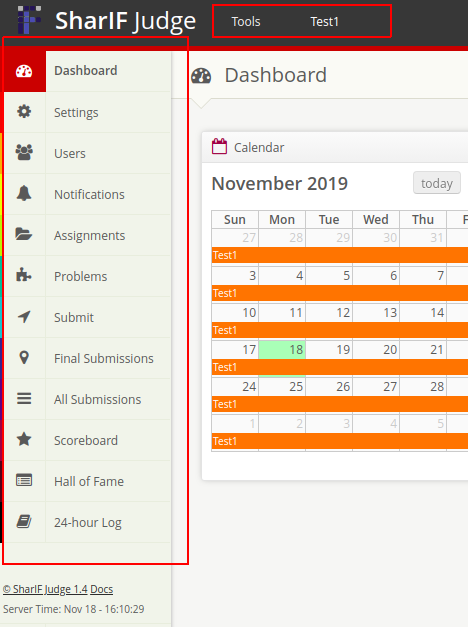
\includegraphics[scale=0.5]{kepatuhan_2_4_5}  
			\caption[Kriteria Sukses 2.4.5 - Menemukan Halaman Web Pada Navigasi]{Kriteria Sukses 2.4.5 - Menemukan Halaman Web Pada Navigasi} 
			\label{fig:kepatuhan_2_4_5} 
		\end{figure}
		
		\subsubsection*{Kriteria Sukses 2.4.6 Headings and Labels}
		\label{subsubsec:kepatuhan_kriteria_2.4.6}
		(Tidak Sukses) \\
		
		Kriteria ini tidak sukses dipatuhi karena :
		\begin{itemize}
			\item Pada halaman \textit{Add User} ada \textit{field input} yang tidak memiliki label yang menjelaskan tujuannya. Pada potongan kode \ref{ls_kepatuhan_2_4_6_add_user} ada bidang masukan yang tidak memiliki label.
			\begin{lstlisting}[basicstyle=\ttfamily, frame=single,
			columns=fullflexible, keepspaces=true, breaklines=true, label=ls_kepatuhan_2_4_6_add_user, caption=Kriteria Sukses 2.4.6 - Halaman \textit{Add User}]
			...
			<p class="input_p">
			<textarea name="new_users" id="new_users" rows="20" cols="80" class="sharif_input">
			# Lines starting with a # sign are comments.
			...
			\end{lstlisting}
			
			\item Pada halaman \textit{Add Assignment} ada \textit{field input} yang tidak memiliki label yang menjelaskan tujuannya. Pada potongan kode \ref{ls_kepatuhan_2_4_6_add_assignment} ada bidang masukan yang tidak memiliki label.
			\begin{lstlisting}[basicstyle=\ttfamily, frame=single,
			columns=fullflexible, keepspaces=true, breaklines=true, label=ls_kepatuhan_2_4_6_add_assignment, caption=Kriteria Sukses 2.4.6 - Halaman \textit{Add Assignment}]
			...
			<td><input type="text" name="name[]" class="sharif_input short" value="{{ problem.name }}"/></td>
			...
			\end{lstlisting}
			
			\item Pada halaman \textit{Problems} bagian \textit{Edit Markdown} dan \textit{Edit Plain HTML} memiliki \textit{field input} yang tidak memiliki label yang menjelaskan tujuannya. Pada potongan kode \ref{ls_kepatuhan_2_4_6_edit_markdown} ada bidang masukan yang tidak memiliki label.
			\begin{lstlisting}[basicstyle=\ttfamily, frame=single,
			columns=fullflexible, keepspaces=true, breaklines=true, label=ls_kepatuhan_2_4_6_edit_markdown, caption=Kriteria Sukses 2.4.6 - Halaman \textit{Problems} bagian \textit{Edit Markdown}]
			...
			<p class="input_p">
			<textarea name="text">{{ problem.description }}</textarea>
			</p>
			...
			\end{lstlisting}
			
		\end{itemize}
		
		\subsubsection*{Kriteria Sukses 2.4.7 Focus Visible}
		\label{subsubsec:kepatuhan_kriteria_2.4.7}
		(Tidak Sukses) \\
		
		Kriteria ini tidak sukses dipatuhi karena fokus tidak tampak ketika fokus sedang berada pada menu \textit{sidebar}.
		
		\subsubsection*{Kriteria Sukses 2.4.8 Location}
		\label{subsubsec:kepatuhan_kriteria_2.4.8}
		(Sukses) \\
		
		Kriteria ini sukses dipatuhi karena pada setiap halaman aplikasi \textit{SharIF Judge} terdapat judul yang menjelaskan lokasi pengguna.
		
		\subsubsection*{Kriteria Sukses 2.4.9 Link Purpose (Link Only)}
		\label{subsubsec:kepatuhan_kriteria_2.4.9}
		(Tidak Sukses) \\
		
		Kriteria ini tidak sukses dipatuhi karena :
		\begin{itemize}
			\item Pada halaman \textit{Assignment} ada gambar yang memiliki tautan tetapi tidak ada teks yang menjelaskan tujuan dari tautan tersebut. Pada potongan kode \ref{ls_kepatuhan_2_4_9_assignment} ditunjukkan bahwa gambar pdf memiliki tautan yang tidak memiliki teks yang menjelaskan tujuannya.
			\begin{lstlisting}[basicstyle=\ttfamily, frame=single,
			columns=fullflexible, keepspaces=true, breaklines=true, label=ls_kepatuhan_2_4_9_assignment, caption=Kriteria Sukses 2.4.9 - Gambar PDF]
			...
			<td>
			<a href="{{ site_url('assignments/pdf/'~item.id) }}"><img src="{{ base_url('assets/images/pdf.svg') }}" /></a>
			</td>
			...
			\end{lstlisting}
			
			\item Pada menu \textit{Top Bar} ada gambar yang memiliki tautan tetapi tidak ada teks yang menjelaskan tujuan dari tautan tersebut. Pada potongan kode \ref{ls_kepatuhan_2_4_9_top_bar} ditunjukkan bahwa gambar logo profil memiliki tautan yang tidak memiliki teks yang menjelaskan tujuannya.
			\begin{lstlisting}[basicstyle=\ttfamily, frame=single,
			columns=fullflexible, keepspaces=true, breaklines=true, label=ls_kepatuhan_2_4_9_top_bar, caption=Kriteria Sukses 2.4.9 - Gambar Logo Profile]
			...
			<a href="{{ site_url('profile') }}" id="profile_link"><i class="fa fa-user"></i></a>
			...
			\end{lstlisting}
			
		\end{itemize}
		
		\subsubsection*{Kriteria Sukses 2.4.10 Section Headings}
		\label{subsubsec:kepatuhan_kriteria_2.4.10}
		(Tidak Sukses) \\
		
		Kriteria ini tidak sukses dipatuhi karena pada aplikasi \textit{SharIF Judge} judul bagian tidak dipakai untuk mengatur konten. Pada potongan kode \ref{ls_kepatuhan_2_4_10_section_headings} bagian judul bagian tidak menggunakan tag \textit{heading}.
		\begin{lstlisting}[basicstyle=\ttfamily, frame=single,
		columns=fullflexible, keepspaces=true, breaklines=true, label=ls_kepatuhan_2_4_10_section_headings, caption=Kriteria Sukses 2.4.10 - Title Heading]
		...
		<div id="page_title">
		<i class="fa "></i>
		<span dir="auto"></span>
		
		</div>
		...
		\end{lstlisting}
		
		\subsubsection*{Kriteria Sukses 2.5.1 Pointer Gestures}
		\label{subsubsec:kepatuhan_kriteria_2.5.1}
		(Sukses) \\
		
		Kriteria ini sukses dipatuhi karena pada aplikasi \textit{SharIF Judge} tidak ada fungsionalitas yang harus dijalankan dengan menggunakan \textit{multipoint} atau gestur berbasis \textit{path}.
		
		\subsubsection*{Kriteria Sukses 2.5.2 Pointer Cancellation}
		\label{subsubsec:kepatuhan_kriteria_2.5.2}
		(Sukses) \\
		
		Kriteria ini sukses dipatuhi karena pada aplikasi \textit{SharIF Judge} tidak ada fungsionalitas yang dapat dioperasikan dengan pointer tunggal dijalankan dengan menggunakan \textit{down-event}.
		
		\subsubsection*{Kriteria Sukses 2.5.3 Label in Name}
		\label{subsubsec:kepatuhan_kriteria_2.5.3}
		(Sukses) \\
		
		Kriteria ini sukses dipatuhi karena pada aplikasi \textit{SharIF Judge} komponen dengan label yang menyertakan teks atau gambar teks, nama tersebut berisi teks yang ditampilkan secara visual.
		
		\subsubsection*{Kriteria Sukses 2.5.4 Motion Actuation}
		\label{subsubsec:kepatuhan_kriteria_2.5.4}
		(Sukses) \\
		
		Kriteria ini sukses dipatuhi karena pada aplikasi \textit{SharIF Judge} tidak terdapat fungsionalitas yang dapat dioperasikan oleh gerakan perangkat atau gerakan pengguna.
		
		\subsubsection*{Kriteria Sukses 2.5.5 Target Size}
		\label{subsubsec:kepatuhan_kriteria_2.5.5}
		(Tidak Sukses) \\
		
		Kriteria ini tidak sukses dipatuhi karena pada aplikasi \textit{SharIF Judge} masih banyak target yang dapat difokus berukuran kurang dari 44 piksel \textit{css}. Salah satu contohnya adalah bidang masukan \textit{Upload Size Limit} yang berukuran 30 piksel css. Tampilan halaman web dapat dilihat pada gambar \ref{fig:kepatuhan_2_5_5}.
		
		\begin{figure}[H]
			\centering  
			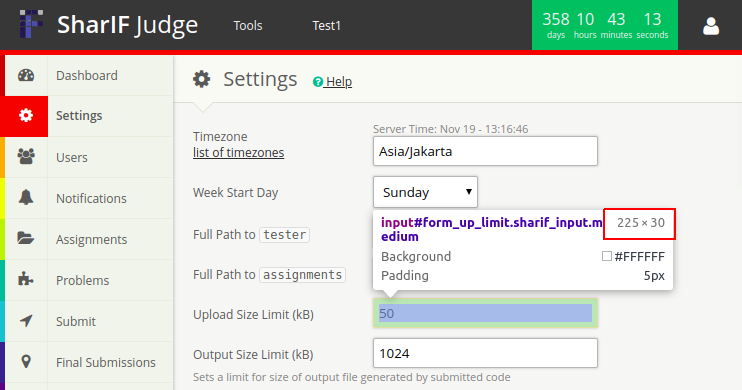
\includegraphics[scale=0.5]{kepatuhan_2_5_5}  
			\caption[Kriteria Sukses 2.5.5 - Bidang Masukan Berukuran 30 css Piksel]{Kriteria Sukses 2.5.5 - Bidang Masukan Berukuran 30 css Piksel} 
			\label{fig:kepatuhan_2_5_5} 
		\end{figure}
		
		\subsubsection*{Kriteria Sukses 2.5.6 Concurrent Input Mechanisms}
		\label{subsubsec:kepatuhan_kriteria_2.5.6}
		(Sukses) \\
		
		Kriteria ini sukses dipatuhi karena pada aplikasi \textit{SharIF Judge} tidak membatasi modalitas masukan yang tersedia pada platform.
		
		\subsection*{\textit{Understandable}}
		\label{subsec:kepatuhan_understandable}
		
		\subsubsection*{Kriteria Sukses 3.1.1 Language of Page}
		\label{subsubsec:kepatuhan_kriteria_3.1.1}
		(Tidak Sukses) \\
		
		Kriteria ini tidak sukses dipatuhi karena elemen \textit{html} tidak memiliki atribut \textit{lang}. Pada potongan kode \ref{ls_kepatuhan_3_1_1} ditunjukkan bahwa elemen \textit{html} tidak memiliki atribut \textit{lang}.
		\begin{lstlisting}[basicstyle=\ttfamily, frame=single,
		columns=fullflexible, keepspaces=true, breaklines=true, label=ls_kepatuhan_3_1_1, caption=Kriteria Sukses 3.1.1 - Elemen \textit{HTML}]
		...
		<html>
		<head>
		...
		\end{lstlisting}
		
		\subsubsection*{Kriteria Sukses 3.1.2 Language of Parts}
		\label{subsubsec:kepatuhan_kriteria_3.1.2}
		(Tidak Sukses) \\
		
		Kriteria ini tidak sukses dipatuhi karena elemen \textit{html} tidak memiliki atribut \textit{lang}. Semua halaman pada aplikasi \textit{SharIF Judge} memakai bahasa Inggris, jika elemen \textit{html} memiliki atribut \textit{lang} maka kriteria ini akan terpenuhi.
		
		\subsubsection*{Kriteria Sukses 3.1.3 Unusual Words}
		\label{subsubsec:kepatuhan_kriteria_3.1.3}
		(Sukses) \\
		
		Kriteria ini sukses dipatuhi karena pada aplikasi \textit{SharIF Judge} tidak ada kata atau frasa tertentu yang digunakan dengan cara tidak biasa atau terbatas. 
		
		\subsubsection*{Kriteria Sukses 3.1.4 Abbreviations}
		\label{subsubsec:kepatuhan_kriteria_3.1.4}
		(Sukses) \\
		
		Kriteria ini sukses dipatuhi karena singkatan yang ada pada \textit{SharIF Judge} lazim digunakan oleh kalangan informatika, singkatan yang dimaksud adalah IP, PDF.
		
		\subsubsection*{Kriteria Sukses 3.1.5 Reading Level}
		\label{subsubsec:kepatuhan_kriteria_3.1.5}
		(Sukses) \\
		
		Kriteria ini sukses dipatuhi karena pada aplikasi \textit{SharIF Judge} tidak ada teks yang membutuhkan kemampuan membaca lebih maju daripada tingkat pendidikan menengah bawah.
		
		\subsubsection*{Kriteria Sukses 3.1.6 Pronunciation}
		\label{subsubsec:kepatuhan_kriteria_3.1.6}
		(Sukses) \\
		
		Kriteria ini sukses dipatuhi karena pada halaman aplikasi \textit{SharIF Judge} setiap kata dapat dimengerti artinya tanpa pengguna perlu mengetahui cara mengucapkan kata tersebut.
		
		\subsubsection*{Kriteria Sukses 3.2.1 On Focus}
		\label{subsubsec:kepatuhan_kriteria_3.2.1}
		(Sukses) \\
		
		Kriteria ini sukses dipatuhi karena pada halaman aplikasi \textit{SharIF Judge} setiap komponen antarmuka yang menerima fokus tidak menyebabkan perubahan konteks.
		
		\subsubsection*{Kriteria Sukses 3.2.2 On Input}
		\label{subsubsec:kepatuhan_kriteria_3.2.2}
		(Sukses) \\
		
		Kriteria ini sukses dipatuhi karena pada setiap pengguna mengubah setelan komponen antarmuka tidak menyebabkan perubahan konteks.
		
		\subsubsection*{Kriteria Sukses 3.2.3 Consistent Navigation}
		\label{subsubsec:kepatuhan_kriteria_3.2.3}
		(Sukses) \\
		
		Kriteria ini sukses dipatuhi karena bagian navigasi menu yang muncul berulang pada tiap halaman aplikasi \textit{SharIF Judge}, muncul dalam urutan relatif yang sama setiap kali terlihat.
		
		\subsubsection*{Kriteria Sukses 3.2.4 Consistent Identification}
		\label{subsubsec:kepatuhan_kriteria_3.2.4}
		(Tidak Sukses) \\
		
		Kriteria ini tidak sukses dipatuhi karena ada komponen yang memiliki fungsi yang sama tetapi tidak diidentifikasi secara konsisten. Komponen tersebut antara lain :
		
		\begin{itemize}
			\item Pada halaman \textit{Assignments} istilah untuk menambah \textit{Assignment} diberi nama \textit{Add}. Tampilan halaman web dapat dilihat pada gambar \ref{fig:kepatuhan_3_2_4_assignments}.
			\begin{figure}[H]
				\centering  
				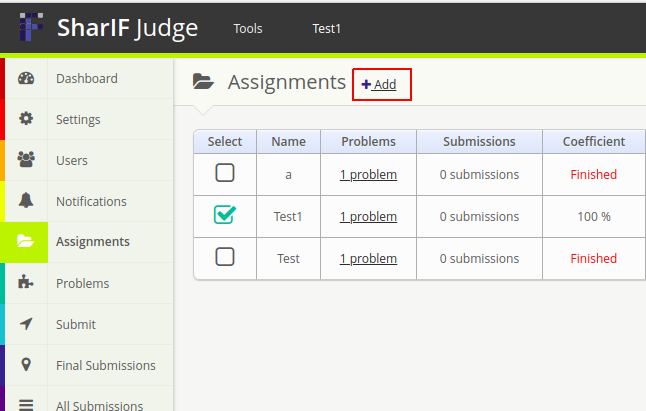
\includegraphics[scale=0.5]{kepatuhan_3_2_4_assignments}  
				\caption[Kriteria Sukses 3.2.4 - \textit{Assignments}]{Kriteria Sukses 3.2.4 - \textit{Assignments}} 
				\label{fig:kepatuhan_3_2_4_assignments} 
			\end{figure}
			
			\item Pada halaman \textit{Users} istilah untuk menambah \textit{user} diberi nama \textit{Add User}. Tampilan halaman web dapat dilihat pada gambar \ref{fig:kepatuhan_3_2_4_users}.
			\begin{figure}[H]
				\centering  
				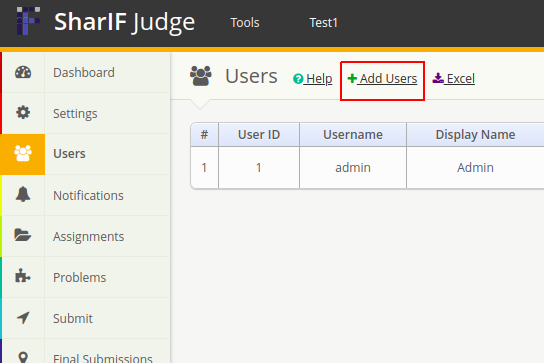
\includegraphics[scale=0.5]{kepatuhan_3_2_4_users}  
				\caption[Kriteria Sukses 3.2.4 - \textit{Users}]{Kriteria Sukses 3.2.4 - \textit{Users}} 
				\label{fig:kepatuhan_3_2_4_users} 
			\end{figure}
			
			\item Pada halaman. \textit{Notifications} istilah untuk menambah \textit{Notification} diberi nama \textit{New}. Tampilan halaman web dapat dilihat pada gambar \ref{fig:kepatuhan_3_2_4_notifications}.
			\begin{figure}[H]
				\centering  
				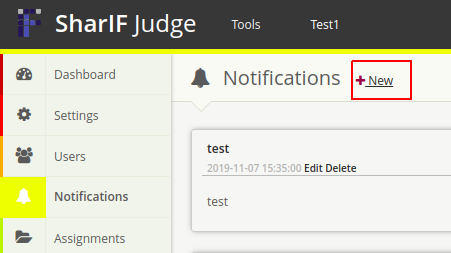
\includegraphics[scale=0.5]{kepatuhan_3_2_4_notifications}  
				\caption[Kriteria Sukses 3.2.4 - \textit{Notifications}]{Kriteria Sukses 3.2.4 - \textit{Notifications}} 
				\label{fig:kepatuhan_3_2_4_notifications} 
			\end{figure}
			
		\end{itemize}
		
		\subsubsection*{Kriteria Sukses 3.2.5 Change on Request}
		\label{subsubsec:kepatuhan_kriteria_3.2.5}
		(Sukses) \\
		
		Kriteria ini sukses dipatuhi karena perubahan konteks hanya terjadi bila dilakukan oleh pengguna.
		
		\subsubsection*{Kriteria Sukses 3.3.1 Error Identification}
		\label{subsubsec:kepatuhan_kriteria_3.3.1}
		(Sukses)\\
		
		Kriteria ini sukses dipatuhi karena kesalahan masukan terdeteksi secara otomatis, \textit{item} yang salah diidentifikasi dan kesalahan tersebut dijelaskan kepada pengguna dalam teks.
		
		\subsubsection*{Kriteria Sukses 3.3.2 Labels or Instructions}
		\label{subsubsec:kepatuhan_kriteria_3.3.2}
		(Tidak Sukses) \\
		
		Kriteria ini tidak sukses karena pada halaman problem bagian edit html, edit markdown, dan edit plain html tidak ada label atau instruksi untuk pengisiannya. Salah satu contoh tampilan halaman web dapat dilihat pada gambar \ref{fig:kepatuhan_3_3_2_edit_markdown}.
		\begin{figure}[H]
			\centering  
			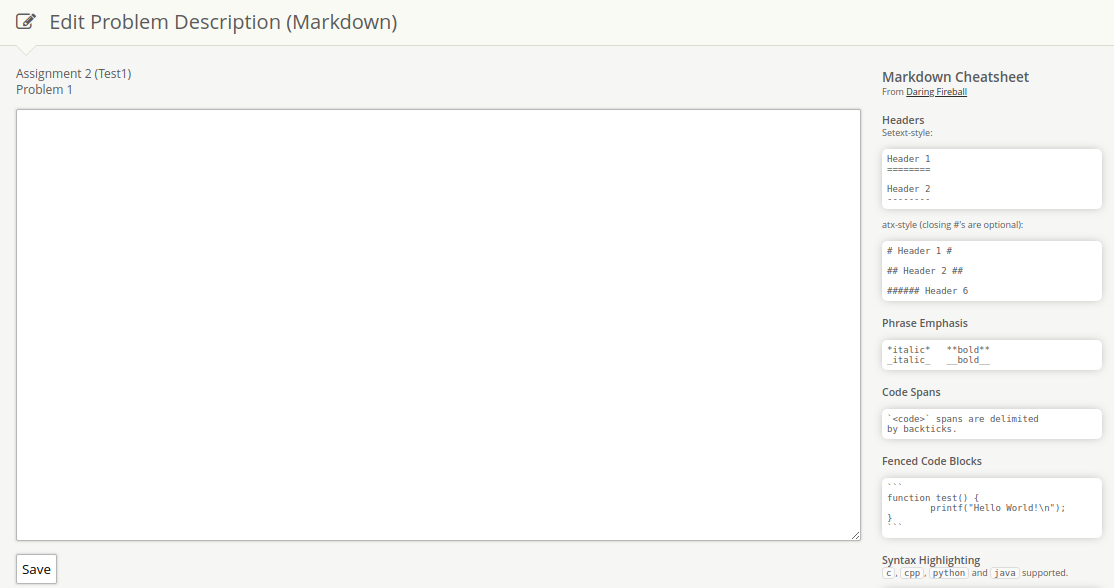
\includegraphics[scale=0.25]{kepatuhan_3_3_2_edit_markdown}  
			\caption[Kriteria Sukses 3.3.2 - \textit{Edit Markdown} Tidak Diberi Label Atau Instruksi]{Kriteria Sukses 3.3.2 - \textit{Edit Markdown} Tidak Diberi Label Atau Instruksi} 
			\label{fig:kepatuhan_3_3_2_edit_markdown} 
		\end{figure}
		
		\subsubsection*{Kriteria Sukses 3.3.3 Error Suggestion}
		\label{subsubsec:kepatuhan_kriteria_3.3.3}
		(Sukses) \\
		
		Kriteria ini sukses dipatuhi karena ketika kesalahan masukan terdeteksi secara otomatis dan saran untuk mengoreksi diketahui, maka saran tersebut diberikan kepada pengguna.
		
		\subsubsection*{Kriteria Sukses 3.3.4 Error Prevention (Legal, Financial, Data)}
		\label{subsubsec:kepatuhan_kriteria_3.3.4}
		(Sukses) \\
		
		Kriteria ini sukses dipatuhi karena pada halaman yang mengirim tanggapan pengguna, data yang dimasukkan oleh pengguna diperiksa terkait kesalahan masukan dan pengguna dipersilakan untuk mengoreksinya.
		
		\subsubsection*{Kriteria Sukses 3.3.5 Help}
		\label{subsubsec:kepatuhan_kriteria_3.3.5}
		(Tidak Sukses) \\
		
		Kriteria ini tidak sukses dipatuhi karena
		pada aplikasi \textit{SharIF Judge} masih ada konten yang tidak diberi label. Pengguna harus dapat mengetahui tujuan dari konten melalui labelnya.
		
		\subsubsection*{Kriteria Sukses 3.3.6 Error Prevention (All)}
		\label{subsubsec:kepatuhan_kriteria_3.3.6}
		(Sukses) \\
		
		Kriteria ini sukses dipatuhi karena pada halaman yang mengharuskan pengguna untuk mengirimkan informasi, data yang dimasukkan oleh pengguna diperiksa terkait kesalahan masukan dan pengguna dipersilakan untuk mengoreksinya.
		
		\subsection*{\textit{Robust}}
		\label{subsec:kepatuhan_robust}
		
		\subsubsection*{Kriteria Sukses 4.1.1 Parsing}
		\label{subsubsec:kepatuhan_kriteria_4.1.1}
		
		\subsubsection*{Kriteria Sukses 4.1.2 Name, Role, Value}
		\label{subsubsec:kepatuhan_kriteria_4.1.2}
		(Tidak Sukses) \\
		
		Kriteria ini tidak sukses dipatuhi karena : 
		\begin{itemize}
			\item Teknologi bantuan tidak dapat mengambil informasi pada \textit{sidebar} karena tidak ada teks yang menjelaskan link tersebut.
		\end{itemize}
		
		\subsubsection*{Kriteria Sukses 4.1.3 Status Messages}
		\label{subsubsec:kepatuhan_kriteria_4.1.3}
		(Tidak Sukses) \\
		
		Kriteria ini tidak sukses dipatuhi karena pada aplikasi \textit{SharIF Judge} tidak ada notifikasi saat melakukan aksi.

		\item \textbf{Menulis dokumen skripsi}\\
		{\bf Status :} Ada sejak rencana kerja skripsi.\\
		{\bf Hasil :} Dokumen skripsi yang sudah dibuat sampai Bab 3.

	\end{enumerate}

\section{Pencapaian Rencana Kerja}
Langkah-langkah kerja yang berhasil diselesaikan dalam Skripsi 1 ini adalah sebagai berikut:
\begin{enumerate}
\item Melakukan studi literatur mengenai WCAG 2.1.
\item Mempelajari struktur dan fitur SharIF Judge.
\item Mengukur tingkat kepatuhan SharIF Judge terhadap WCAG 2.1.
\item Membuat dokumen skripsi.
\end{enumerate}



\section{Kendala yang Dihadapi}
%TULISKAN BAGIAN INI JIKA DOKUMEN ANDA TIPE A ATAU C
Kendala - kendala yang dihadapi selama mengerjakan skripsi :
\begin{itemize}
	\item Proses instalasi aplikasi \textit{SharIF Judge} sulit dilakukan sehingga memerlukan bantuan admin.
	\item Mempelajari \textit{framework} yang dipakai pada aplikasi \textit{SharIF Judge}.
	\item Sulit memahami pedoman yang ada pada \textit{WCAG 2.1} karena isinya berbahasa Inggris yang bersifat teknis.
\end{itemize}

\vspace{1cm}
\centering Bandung, \tanggal\\
\vspace{2cm} \nama \\ 
\vspace{1cm}

Menyetujui, \\
\ifdefstring{\jumpemb}{2}{
\vspace{1.5cm}
\begin{centering} Menyetujui,\\ \end{centering} \vspace{0.75cm}
\begin{minipage}[b]{0.45\linewidth}
% \centering Bandung, \makebox[0.5cm]{\hrulefill}/\makebox[0.5cm]{\hrulefill}/2013 \\
\vspace{2cm} Nama: \pembA \\ Pembimbing Utama
\end{minipage} \hspace{0.5cm}
\begin{minipage}[b]{0.45\linewidth}
% \centering Bandung, \makebox[0.5cm]{\hrulefill}/\makebox[0.5cm]{\hrulefill}/2013\\
\vspace{2cm} Nama: \pembB \\ Pembimbing Pendamping
\end{minipage}
\vspace{0.5cm}
}{
% \centering Bandung, \makebox[0.5cm]{\hrulefill}/\makebox[0.5cm]{\hrulefill}/2013\\
\vspace{2cm} Nama: \pembA \\ Pembimbing Tunggal
}
\end{document}

